\documentclass[twocolumn]{article}

%% ====================================================================
%% Packages
%% ====================================================================
\usepackage[T1]{fontenc}
\usepackage[utf8]{inputenc}
\usepackage{textcomp}
\usepackage{graphicx}
\usepackage{url}
\usepackage{amsmath}
\usepackage{amssymb}
\usepackage{amsfonts}
\usepackage{xcolor}
\usepackage{array}
\usepackage{float}
\usepackage{subcaption}
\usepackage{caption}
\usepackage{booktabs}
\usepackage{geometry}
\usepackage{multirow}
\usepackage{placeins}
\usepackage{hyperref}
\geometry{margin=2.5cm}
\usepackage{authblk}
\usepackage{enumitem}
\usepackage{algorithm}
\usepackage{algpseudocode}
\usepackage{tikz}
\usetikzlibrary{shapes.geometric,arrows.meta,positioning,fit,backgrounds,calc}

%%
\title{Fine-Tuning Vision-Language Models for\\
Understanding Bridge Damage and Scoring Repair Priority:\\
\large Application Methodology}

\author[1]{Takato Yasuno}
% \affil[1]{Affiliation}
% \affil[ ]{Email: }

\date{2026}

\begin{document}

\renewcommand{\abstractname}{Abstract}
\renewcommand{\refname}{References}
\renewcommand{\figurename}{Figure}
\renewcommand{\tablename}{Table}

\maketitle

%% ====================================================================
\begin{abstract}
%% ====================================================================

Bridge inspection in Japan requires mandatory visual assessments every five years,
yet qualitative damage ratings (levels a--e) assigned by different engineers exhibit
significant inter-rater variability---a critical barrier to consistent infrastructure
management. The aging of skilled engineers further threatens inspection capacity.
This paper presents a methodology for automating bridge damage understanding and
repair priority scoring using fine-tuned Vision-Language Models (VLMs).

We fine-tune LLaVA-1.5-7B with QLoRA (4-bit NF4 quantization, rank=32) on
up to 4{,}000 paired bridge damage images and inspection text records, then
evaluate on a fixed test set of 800 images. The model outputs natural language
descriptions identifying structural members and damage patterns, from which
a rule-based scoring engine calculates a five-level repair priority index.
A progressive training study (1k/2k/3k/4k samples) reveals that 2k training
samples achieve near-optimal validation loss (3.073) with only 2.9 hours of
training, exhibiting diminishing returns beyond this scale.
Inference optimization combining \texttt{torch.compile()} and batch processing
(batch\_size=8) achieves 10.06 seconds per image---a 70.2\% reduction over the
unoptimized baseline.

Our approach contributes to data governance in bridge inspection, reduces
inter-rater variability, and provides AI-assisted triage to augment
expert engineers in inspection workflows.

\end{abstract}

\noindent
\textbf{Keywords:} Vision-Language Models, Fine-Tuning, QLoRA, Bridge Inspection,
Damage Assessment, Repair Priority Scoring, Infrastructure AI.

\noindent
\textbf{Code}: \url{https://github.com/tk-yasuno/damage_vlm_finetune}

%% ====================================================================
\section{Introduction}
\label{sec:introduction}
%% ====================================================================

Japan's road network encompasses approximately 730{,}000 highway bridges,
of which nearly half will exceed 50 years of service life by
2033~\cite{mlit2023bridge}.
Under the Road Act (amended 2014), every road bridge must undergo close-up
visual inspection every five years, producing paired records: a photographic
image of the damage site and a hand-written inspection note (\textit{shoken})
describing the structural member, damage type, severity, and recommended
corrective action.

Despite this systematic framework, two persistent challenges impede inspection
quality.
\textbf{Inter-rater variability:} damage ratings (levels a--e) assigned by
different engineers diverge due to subjective judgment, undermining data
consistency across the national bridge stock~\cite{mlit2023bridge}.
\textbf{Workforce contraction:} experienced bridge inspectors are retiring
faster than they can be replaced, threatening capacity at the required cadence.

Recent Vision-Language Models (VLMs) present a promising path forward.
Models such as LLaVA~\cite{liu2024llava},
InstructBLIP~\cite{dai2023instructblip}, and GPT-4V~\cite{openai2023gpt4}
can generate detailed descriptive text from images; however, these
general-purpose models have no exposure to specialised Japanese inspection
vocabulary and cannot produce the structured output required by inspection
standards.

This paper presents a methodology for \textbf{bridge damage understanding and
repair priority scoring} via domain-adapted VLMs.
We fine-tune LLaVA-1.5-7B~\cite{liu2024llava} with
QLoRA~\cite{dettmers2023qlora} on up to 4{,}000 paired bridge inspection
records and deploy a rule-based scoring engine that produces a five-level
repair priority index (Immediate to Minimal).

\textbf{Contributions:}
\begin{enumerate}[leftmargin=*,itemsep=1pt]
  \item \textbf{Damage VLM}: the first QLoRA fine-tuning study of a
        7B-parameter VLM on Japanese bridge inspection image--text pairs,
        achieving the \textit{Acceptable} quality tier on a consumer GPU.
  \item \textbf{Repair Priority Scoring}: a transparent, auditable rule engine
        that converts VLM free-form output into a five-level priority index,
        enabling consistent maintenance triage without subjective judgment.
  \item \textbf{Visual Inspection ScoreBot}: an end-to-end local pipeline
        combining the Damage VLM with the scoring engine---deployable without
        cloud API dependencies on a single consumer GPU.
\end{enumerate}

This work builds on the authors' prior study of quantized LLaVA-1.5-7B for
bridge damage assessment~\cite{yasuno2026quantized}, which benchmarked
INT4/INT8/BF16 quantization levels without task-specific fine-tuning.
The multi-stage inspection framework in~\cite{yasuno2026multistage} further
motivated the end-to-end pipeline presented here.

Section~\ref{sec:related} reviews related work.
Section~\ref{sec:methodology} details the system methodology.
Section~\ref{sec:results} presents evaluation results.
Section~\ref{sec:discussion} discusses findings and limitations.
Section~\ref{sec:conclusion} concludes.

%% ====================================================================
\section{Related Work}
\label{sec:related}
%% ====================================================================

\subsection{Vision-Language Models for Structural Damage Understanding}

The development of large VLMs accelerated with CLIP~\cite{radford2021clip},
which established scalable joint image--text representation via contrastive
pre-training on 400 million web image--caption pairs.
Flamingo~\cite{alayrac2022flamingo} extended this to few-shot visual reasoning
by conditioning frozen language models on visual features through gated
cross-attention layers.
BLIP-2~\cite{li2023blip2} and InstructBLIP~\cite{dai2023instructblip} improved
instruction-following by bridging frozen image encoders and language models
via a lightweight querying transformer.
LLaVA~\cite{liu2024llava} simplified the paradigm by projecting visual tokens
directly into a language model embedding space, enabling visual instruction
tuning at reduced cost.
Its successor LLaVA-1.5~\cite{liu2024llava15}, a CVPR~2024 highlight paper,
showed that an MLP connector with CLIP-ViT-L-336\,px achieves state-of-the-art
across 11 benchmarks using only 1.2\,M publicly available training samples
--- the same base model adopted in this work.
MiniGPT-4~\cite{zhu2024minigpt4} demonstrated that aligning a frozen visual
encoder with a large language model through a single projection layer suffices
for rich image-description generation.

Foundational perception models have further expanded the toolkit for inspection.
Segment Anything (SAM)~\cite{kirillov2023sam} introduced a promptable model
trained on over one billion masks that transfers zero-shot across diverse
visual domains.
Grounding DINO~\cite{liu2023groundingdino} combined transformer-based detection
with language grounding for open-set localisation, complementary to the
language-generation focus of generative VLMs.

In civil infrastructure, vision-based inspection has followed an independent
trajectory focused on pixel-level detection.
Cha et al.~\cite{cha2017deepcrack} demonstrated that convolutional neural
networks detect surface cracks with near-expert accuracy.
Spencer et al.~\cite{spencer2019vision} surveyed computer vision advances for
structural inspection, noting the gap between pixel-level detection and the
natural language reporting required in engineering practice.
Dorafshan et al.~\cite{dorafshan2018concrete} benchmarked CNN detectors for
concrete crack localisation, and Hsieh and Tsai~\cite{hsieh2020concrete}
compared machine learning approaches for crack detection.

Our work bridges these two streams: task-specific QLoRA fine-tuning of
LLaVA-1.5 generates the structured natural language output required by
Japanese inspection standards, going beyond pixel-level detection to holistic
damage description in domain-appropriate Japanese vocabulary.
Early work on few-shot damage vision mining~\cite{yasuno2023fewshot}
showed that imbalanced data and rare damage events are fundamental
challenges in infrastructure inspection datasets.
A multi-stage bridge inspection system~\cite{yasuno2026multistage} integrated
foundation models with location anonymisation for privacy-preserving
field imaging.
Our quantization study~\cite{yasuno2026quantized} benchmarked inference
speed and description quality across LLaVA-1.5-7B precision levels,
establishing INT4 QLoRA as the optimal speed--quality trade-off
and motivating the domain fine-tuning step presented in this paper.

\subsection{AI-Assisted Decision Support for Infrastructure Maintenance}

Bridge management has long relied on formal decision-support frameworks.
Frangopol~\cite{frangopol2011lifecycle} formalised life-cycle performance
optimisation for structural systems under uncertainty, establishing the
theoretical basis for risk-based inspection prioritisation.
Operational bridge management systems encode engineering heuristics into
rule-based priority scores but depend on consistent structured input that
manual inspection cannot always guarantee.

Yang et al.~\cite{yang2018dam} applied deep CNNs to automatically map surface
cracks on dam structures, reducing manual effort in routine assessments.
Such detection-focused systems, however, lack the semantic understanding
needed to recommend maintenance actions or to assign priority across
heterogeneous damage types.

More recently, vision-language models have been adapted for zero-shot
industrial inspection.
WinCLIP~\cite{jeong2023winclip} (CVPR~2023) introduced a compositional
ensemble on window/patch/image-level CLIP features, achieving 91.8\% AUROC
in zero-shot anomaly classification on MVTec-AD without task-specific training.
AnomalyCLIP~\cite{zhou2024anomalyclip} (ICLR~2024) extended this line by
learning object-agnostic text prompts that capture generic normality and
abnormality, enabling strong zero-shot transfer across 17 datasets spanning
defect inspection and medical imaging.
AnomalyGPT~\cite{gu2024anomalygpt} (AAAI~2024) demonstrated that large
vision-language models fine-tuned with simulated anomalous images and
corresponding textual descriptions achieve state-of-the-art industrial
anomaly detection without manual threshold setting, reaching 94.1\% image-level
AUC with only one normal reference shot.

Our scoring engine addresses the bridge-specific gap: rather than detecting
anomalies from scratch, it consumes VLM-generated Japanese damage descriptions
and applies YAML-defined weights for member type, severity, location, and
extent to produce a five-level repair priority index.
Domain experts can audit and update the scoring logic without machine learning
expertise, preserving transparency for safety-critical decisions.
Complementary work on heterogeneous graph importance scoring for bridge
networks~\cite{yasuno2026graph} demonstrated that LLM-generated
interpretations effectively bridge algorithmic rankings and maintenance
decision-makers, reinforcing the value of language as an interface between
AI outputs and engineering judgment.

\subsection{Multimodal Systems for Industrial Visual Inspection}

The emergence of GPT-4V~\cite{openai2023gpt4} catalysed interest in
general-purpose multimodal systems for industrial applications.
Cao et al.~\cite{cao2023gpt4vanomaly} systematically evaluated GPT-4V on
anomaly detection across four modalities and nine tasks, demonstrating
promising zero-shot and one-shot performance while highlighting limitations
in fine-grained localisation of subtle defects.
Prompt-engineered GPT-4V can identify manufacturing defects and answer
technical questions from product photographs, yet proprietary API dependence,
latency, and data privacy constraints limit deployment in regulated
infrastructure contexts.

Open-source VLMs fine-tuned or adapted for domain-specific inspection offer
a more practical path.
Anomaly-OV~\cite{xu2025anomalyov} (CVPR~2025) proposed a specialist visual
assistant for zero-shot anomaly detection and reasoning, introducing a
Look-Twice Feature Matching mechanism that adaptively emphasises abnormal
visual tokens, achieving significant improvements over generalist MLLMs on
industrial and medical benchmarks.
Zhang et al.~\cite{zhang2025trainingfree} (CVPR~2025) demonstrated
training-free anomaly detection using vision and language foundation models,
eliminating fine-tuning while maintaining competitive performance on standard
benchmarks --- contrasting with our QLoRA-based domain adaptation strategy.
LogicAD~\cite{jin2025logicad} (AAAI~2025) combined VLM-based text feature
extraction with logical reasoning to produce explainable anomaly reports,
aligning with the engineering interpretability requirements of infrastructure
operators.

Our \textbf{Visual Inspection ScoreBot} operationalises this paradigm for
Japanese bridge infrastructure: the Damage VLM generates free-form Japanese
damage descriptions; a regex-based extractor converts them to structured
JSON attributes; and the scoring engine produces actionable priority
scores --- all running locally on a single consumer GPU without external API
calls.
This architecture aligns with emerging industrial AI patterns in which a
language model serves as the semantic front-end to a deterministic rule
engine~\cite{liu2024llava,dettmers2023qlora}, combining interpretability
with the expressive power of neural language understanding.

\subsection{Automation and Robotics in the Construction Domain}

The International Symposium on Automation and Robotics in Construction
(ISARC) provides a focused forum for construction-domain AI, and
contributions from ISARC~2023--2025 reveal three convergent themes
directly relevant to this paper: (i)~language-model-driven extraction
from inspection documents, (ii)~multimodal report generation from visual
data, and (iii)~deep-learning-based structural damage detection coupled
with maintenance scheduling.

\textbf{Language models for inspection document processing.}
Omar and Moselhi~\cite{omar2023bridge} (ISARC~2023) established an
integrated pipeline for automated acquisition and parsing of bridge
inspection reports, demonstrating that text-mining can replace manual
data entry for deck-deficiency records.
Their follow-on study~\cite{omar2025bridge} (ISARC~2025) replaced
rule-based parsing with fine-tuned Generative Pre-trained Transformers,
achieving substantial accuracy gains in recognising concrete-defect
entities from free-text engineering records --- a direct antecedent of
the QLoRA-based Damage VLM strategy presented here, which adapts the
same fine-tuning paradigm to Japanese inspection vocabulary.
Reja et al.~\cite{reja2025llm} (ISARC~2025) compared few-shot LLM
classifiers against fine-tuned transformers for road maintenance log
classification, confirming that domain-adapted language models
consistently outperform general-purpose prompting in specialised
infrastructure contexts.

\textbf{Multimodal and vision-language approaches.}
Pu et al.~\cite{pu2024mllm} (ISARC~2024) employed multimodal large
language models with Set-of-Mark prompting to generate construction
inspection reports directly from annotated site photographs --- the
closest prior work to our Damage VLM pipeline, though targeting
general construction quality in English rather than bridge-specific
damage in Japanese regulatory vocabulary.
Hsu et al.~\cite{hsu2024vlcon} (ISARC~2024) released VL-Con, a
construction-domain vision-language dataset, reinforcing the finding
that task-specific data collection is a prerequisite for reliable VLM
performance in AEC applications and motivating the curated Japanese
instruction dataset described in Section~\ref{sec:dataset}.
Mengiste et al.~\cite{mengiste2025progress} (ISARC~2025) automated
weekly construction progress reporting using multimodal LLM workflows,
further illustrating the industrial demand for language-based interfaces
to visual inspection data.

\textbf{Structural damage detection and maintenance decision support.}
Assad et al.~\cite{assad2025crack} (ISARC~2025) benchmarked
single-stage versus two-stage detectors for bridge crack detection
and segmentation, confirming that pixel-level localisation methods
remain the baseline for damage mapping, though without generating the
natural-language descriptions required for regulatory reporting.
Zuo et al.~\cite{zuo2025transformer} (ISARC~2025) combined
transformer-based detection with multi-resolution 3D reconstruction
to spatially localise bridge surface defects, demonstrating the
complementary role of geometric modelling alongside 2D image-based
language generation.
N\'{u}\~{n}ez Varillas et al.~\cite{nunez2024bridge} (ISARC~2024)
integrated UAV photogrammetry with CNN-based concrete damage
classification on reconstructed bridge 3D models, illustrating
how remote sensing reduces inspector exposure while maintaining
detection accuracy.
At the maintenance-decision level, Alsharqawi et al.~\cite{alsharqawi2025mrr}
(ISARC~2025) proposed an automated scheduling tool for bridge
maintenance, repair, and replacement using multi-objective genetic
algorithms.
Their portfolio-level optimiser is complementary to our inspection-level
priority scoring engine: the five-level repair priority index produced
by the ScoreBot provides the per-element damage state that such
optimisers require as input.

Collectively, these ISARC contributions confirm two transitions in
construction inspection practice: automated language processing is
displacing manual report writing, and multimodal architectures are
superseding single-modality vision pipelines.
The present work advances both transitions by fine-tuning a
state-of-the-art open-source VLM (LLaVA-1.5-7B) on a curated Japanese
bridge inspection dataset, delivering domain-appropriate structured
damage descriptions without dependence on proprietary APIs or
manual post-processing.

%% ====================================================================
\section{Methodology}
\label{sec:methodology}
%% ====================================================================

\subsection{System Architecture Overview}

Figure~\ref{fig:pipeline} illustrates the end-to-end pipeline comprising four
sequential stages: image input, VLM-based damage understanding, structured
information extraction, and repair priority scoring.

%% ------ TikZ Pipeline Figure ------
\begin{figure}[t]
\centering
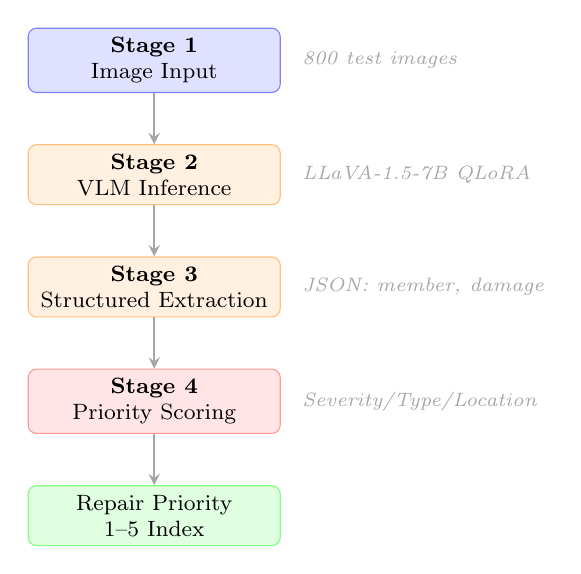
\begin{tikzpicture}[
  node distance=0.65cm and 0.1cm,
  box/.style={rectangle, draw=gray!70, rounded corners=3pt,
              minimum width=3.2cm, minimum height=0.65cm,
              align=center, font=\footnotesize},
  stage/.style={box, fill=blue!12, draw=blue!50},
  proc/.style={box,  fill=orange!12, draw=orange!50},
  score/.style={box, fill=red!10,  draw=red!40},
  outbox/.style={box,   fill=green!12, draw=green!50},
  arr/.style={->, >=stealth, thick, gray!70},
  label/.style={font=\scriptsize\itshape, text=gray!70}
]

\node[stage]  (inp)  {\textbf{Stage 1}\\Image Input};
\node[proc,   below=of inp]  (vlm)  {\textbf{Stage 2}\\VLM Inference};
\node[proc,   below=of vlm]  (ext)  {\textbf{Stage 3}\\Structured Extraction};
\node[score,  below=of ext]  (scr)  {\textbf{Stage 4}\\Priority Scoring};
\node[outbox,    below=of scr]  (outnd)  {Repair Priority\\1--5 Index};

\draw[arr] (inp) -- (vlm);
\draw[arr] (vlm) -- (ext);
\draw[arr] (ext) -- (scr);
\draw[arr] (scr) -- (outnd);

\node[label, right=0.15cm of inp] {800 test images};
\node[label, right=0.15cm of vlm] {LLaVA-1.5-7B QLoRA};
\node[label, right=0.15cm of ext] {JSON: member, damage};
\node[label, right=0.15cm of scr] {Severity/Type/Location};
\end{tikzpicture}
\caption{End-to-end pipeline for bridge damage understanding and repair
         priority scoring. Fine-tuning (Section~\ref{sec:finetuning}) targets
         Stage~2; Stages~3--4 remain rule-based.}
\label{fig:pipeline}
\end{figure}

Table~\ref{tab:components} summarises the technology stack at each stage.

\begin{table}[h]
\centering
\caption{Pipeline component overview.}
\label{tab:components}
\setlength{\tabcolsep}{4pt}
\begin{tabular}{llp{2.6cm}}
\toprule
\textbf{Stage} & \textbf{Component} & \textbf{Technology} \\
\midrule
1. Input        & Image loader        & Python Pillow \\
2. VLM          & Damage description  & LLaVA-1.5-7B QLoRA \\
3. Extraction   & Structured JSON     & Rule-based regex \\
4. Scoring      & Priority index      & YAML rule engine \\
\bottomrule
\end{tabular}
\end{table}

The pipeline is designed to run on consumer-grade GPUs (NVIDIA RTX 4060 Ti 16GB,
CUDA 12.4), enabling practical deployment without data-centre hardware.

%% ====================================================================
\subsection{Dataset Construction}
\label{sec:dataset}
%% ====================================================================

\subsubsection{Source Data}

We collect 10{,}789 paired bridge damage images and Japanese inspection text
records from routine close-up visual inspections conducted under Japan's Road
Act, which mandates five-year periodic bridge inspections.
Each record contains a damage image and the corresponding inspector's \emph{shooken}
(observation text, Japanese: \textit{shoken}) written using standardised civil engineering terminology.

\subsubsection{Quality Filtering}

To ensure training data quality, we apply the following filters:
\begin{itemize}[leftmargin=*,itemsep=1pt]
  \item \textbf{Text length}: 15--500 characters (removes empty and excessively
        verbose records).
  \item \textbf{Invalid patterns}: excludes records containing only placeholder
        text (``nashi'' (none), ``???'', or similar).
  \item \textbf{Keyword requirement}: at least one structural member term
        (e.g., \textit{girder, deck, pier}) and one damage term
        (e.g., \textit{rebar exposure, crack, corrosion}) must be present.
\end{itemize}

\subsubsection{Stratified Sampling and Split Strategy}

After filtering, we construct training and evaluation sets using stratified
sampling by cross-product of member type and damage type to ensure class balance.

\begin{itemize}[leftmargin=*,itemsep=1pt]
  \item \textbf{Fixed test set}: 800 samples drawn with random seed 42, held
        out for all experiments (798 with valid images, 2 missing).
  \item \textbf{Progressive training sets}: independently sampled sets of
        1k, 2k, 3k, and 4k images to study data-scaling behaviour.
        Each training set uses an 80/20 train/validation split.
        This progression follows the scale-search methodology
        in~\cite{yasuno2026japanese}, which identified $n\approx4{,}000$
        as optimal for Japanese domain-specific language models---extended
        here to the multimodal VLM setting.
\end{itemize}

Table~\ref{tab:dataset} shows the resulting dataset statistics.

\begin{table}[h]
\centering
\caption{Dataset statistics after quality filtering.}
\label{tab:dataset}
\begin{tabular}{lrr}
\toprule
\textbf{Split} & \textbf{Images} & \textbf{Valid (\%)} \\
\midrule
Test (fixed)          & 800   & 798 (99.75\%) \\
\midrule
Train-1k (train/val)  & 799 / 200   & 100\% \\
Train-2k (train/val)  & 1{,}599 / 400 & 100\% \\
Train-3k (train/val)  & 2{,}398 / 600 & 100\% \\
Train-4k (train/val)  & 3{,}196 / 799 & 100\% \\
\midrule
Source pool           & 10{,}789 & --- \\
\bottomrule
\end{tabular}
\end{table}

%% ====================================================================
\subsection{QLoRA Fine-Tuning}
\label{sec:finetuning}
%% ====================================================================

\subsubsection{Base Model}

We fine-tune \textbf{LLaVA-1.5-7B}~\cite{liu2024llava} (HuggingFace identifier:
\texttt{llava-hf/llava-1.5-7b-hf}), an instruction-tuned vision-language model
combining CLIP ViT-L/14 as the vision encoder and Vicuna-1.5-7B as the
language decoder connected via a two-layer MLP projection.
LLaVA-1.5-7B is chosen for its strong visual instruction-following capability
and practical size for consumer GPU deployment.

\subsubsection{QLoRA Configuration}

We apply \textbf{QLoRA}~\cite{dettmers2023qlora} (Quantized Low-Rank Adaptation),
which loads the base model in 4-bit NF4 precision while training low-rank adapter
matrices in full precision. This enables fine-tuning a 7B-parameter model within
16GB VRAM.

The quantization configuration uses 4-bit NF4 with double quantization (compressing
quantization constants themselves) via \texttt{bitsandbytes}~\cite{dettmers2022llmint8}.
Low-rank adapters are inserted into all major projection matrices as shown in
Table~\ref{tab:qlora_config}.

\begin{table}[h]
\centering
\caption{QLoRA and training hyperparameters.}
\label{tab:qlora_config}
\begin{tabular}{ll}
\toprule
\textbf{Parameter} & \textbf{Value} \\
\midrule
\multicolumn{2}{l}{\textit{Quantization}} \\
Precision & 4-bit NF4 \\
Double quantization & Enabled \\
Compute dtype & float16 \\
\midrule
\multicolumn{2}{l}{\textit{LoRA Adapters}} \\
Rank $r$ & 32 \\
Alpha $\alpha$ & 64 \\
Dropout & 0.05 \\
Target modules & \texttt{q,k,v,o\_proj;} \\
 & \texttt{gate,up,down\_proj} \\
\midrule
\multicolumn{2}{l}{\textit{Training}} \\
Batch size & 4 \\
Gradient accumulation & 4 (eff.\ batch = 16) \\
Learning rate & $2 \times 10^{-4}$ \\
Epochs & 3 \\
Warmup steps & 50 \\
Max gradient norm & 1.0 \\
Weight decay & 0.01 \\
Optimizer & AdamW \\
LR scheduler & Cosine \\
Mixed precision & FP16 \\
\midrule
\multicolumn{2}{l}{\textit{Hardware}} \\
GPU & RTX 4060 Ti 16GB \\
CUDA & 12.4 \\
PyTorch & 2.6.0+cu124 \\
Transformers & 4.57.6 \\
PEFT & 0.18.1 \\
\bottomrule
\end{tabular}
\end{table}

The adapter scaling factor is $s = \alpha / r = 64/32 = 2$, controlling the
magnitude of the learned residual updates relative to the frozen base weights.
The LoRA decomposition for each weight matrix $W_0 \in \mathbb{R}^{d \times k}$ is:
\begin{equation}
  W = W_0 + \frac{\alpha}{r} \, B A
  \label{eq:lora}
\end{equation}
where $B \in \mathbb{R}^{d \times r}$ and $A \in \mathbb{R}^{r \times k}$ are the
low-rank adapter matrices initialised as $B = \mathbf{0}$ and $A \sim \mathcal{N}(0, \sigma^2)$.

\subsubsection{Progressive Training Strategy}
\label{sec:progressive}

To investigate data-scaling behaviour, we train four independent models on
progressively larger datasets (1k, 2k, 3k, 4k) using identical hyperparameters.
Table~\ref{tab:training_results} reports validation loss and training duration
for each scale.

\begin{table}[h]
\centering
\caption{Progressive training results (LLaVA-1.5-7B QLoRA).}
\label{tab:training_results}
\begin{tabular}{lrrrl}
\toprule
\textbf{Model} & \textbf{Steps} & \textbf{Val Loss} & \textbf{Duration} & \textbf{Best Ckpt} \\
\midrule
1k & 150 & 3.135 & 1:22:57 & step-100 \\
2k & 300 & 3.073 & 2:55:37 & step-300 \\
3k & 450 & 3.073 & 4:31:44 & step-400 \\
4k & 600 & 3.067 & 6:19:10 & step-600 \\
\bottomrule
\end{tabular}
\end{table}

Three key observations emerge:
\begin{enumerate}[leftmargin=*,itemsep=1pt]
  \item \textbf{1k $\to$ 2k}: Validation loss decreases by 1.98\%,
        the largest single-step improvement, confirming benefit of additional data.
  \item \textbf{Plateau at 2k--3k}: Loss stagnates at 3.073 despite 1.6$\times$
        more training time, indicating convergence of the fine-tuning signal.
  \item \textbf{Marginal gain at 4k}: Only 0.2\% improvement over 3k at
        1.4$\times$ cost, demonstrating strong diminishing returns.
\end{enumerate}

The \textbf{2k model} therefore offers the optimal cost--benefit trade-off:
near-maximum accuracy ($\Delta = 0.2\%$ from 4k) achieved in 2.9 hours---2.2$\times$
faster than the 4k baseline.

%% ====================================================================
\subsection{Inference Optimisation}
\label{sec:inference}
%% ====================================================================

Running inference on 800 test images with an unoptimised HuggingFace
\texttt{generate()} call requires 33.79 seconds per image (7.5 hours total),
making systematic multi-model evaluation impractical. We implement three
complementary optimisations.

\subsubsection{\texttt{torch.compile()} Graph Optimisation}

PyTorch 2.0 introduced \texttt{torch.compile()}~\cite{pytorch2023compile},
which applies TorchDynamo bytecode analysis and TorchInductor ahead-of-time
compilation to the model's computation graph.
We use \texttt{mode=\textrm{``}reduce-overhead\textrm{''}}, which
minimises Python interpreter overhead---the dominant bottleneck for repeated
single-batch inference calls.
An initial warm-up batch ($\approx$60--80 seconds) is followed by accelerated
subsequent inference.

\subsubsection{Batch Processing}

We implement a batched inference loop that processes $B$ images simultaneously,
padding inputs to uniform length within each batch:

\begin{equation}
  \hat{T}_{\text{total}} = \underbrace{t_{\text{compile}}}_{\text{once}} +
  \left\lceil \frac{N}{B} \right\rceil \cdot t_{\text{batch}}(B)
  \label{eq:batch_time}
\end{equation}
where $N = 800$ is the test set size and $t_{\text{batch}}(B)$ is the
per-batch latency at batch size $B$.

\subsubsection{Batch Size Selection}

We empirically evaluate batch sizes $B \in \{4, 8, 16\}$ on the RTX 4060 Ti
(16GB VRAM). Table~\ref{tab:batch_opt} reports per-image latency and GPU memory
utilisation.

\begin{table}[h]
\centering
\caption{Batch size optimisation results (2k model, 16 test samples).}
\label{tab:batch_opt}
\begin{tabular}{lrrl}
\toprule
\textbf{Batch} & \textbf{s/image} & \textbf{VRAM} & \textbf{Status} \\
\midrule
Baseline (v0.4) & 33.79 & --- & Reference \\
$B=4$ & 16.80 & $<$80\% & \checkmark \\
$B=8$ & 10.06 & $\approx$78\% & \checkmark\; \textbf{Optimal} \\
$B=16$ & --- & 98\% & OOM risk \\
\bottomrule
\end{tabular}
\end{table}

$B = 8$ reduces per-image latency by 70.2\% relative to the baseline (33.79 $\to$
10.06 seconds) while keeping GPU memory below the 80\% safety threshold.
$B = 16$ saturates VRAM at 15.7/16.0 GB, inducing long \texttt{torch.compile()}
compilation and out-of-memory risk; it is therefore excluded.

\subsubsection{Token Budget Optimisation}

We analyse per-model output token distributions on 40-sample pilot runs to set
\texttt{max\_new\_tokens} without systematic truncation:

\begin{table}[h]
\centering
\caption{Output token statistics by training scale.}
\label{tab:tokens}
\begin{tabular}{lrrl}
\toprule
\textbf{Model} & \textbf{Mean} & \textbf{Std} & \textbf{max\_new\_tokens} \\
\midrule
1k & 348.5 & 148.4 & 512 \\
2k & 279.7 &  84.0 & 384 \\
3k & 266.4 & 160.0 & 384 \\
4k & 231.6 &  70.8 & 384 \\
\bottomrule
\end{tabular}
\end{table}

More training data produces more concise outputs (33.5\% token reduction from
1k to 4k), an inverse-scaling phenomenon we attribute to improved instruction
following. Setting \texttt{max\_new\_tokens}$=384$ eliminates truncation for 2k
and 4k models (10\% and 0\% truncation, respectively) while reducing generation
time by 25\% over the conservative default of 512.

We additionally apply \texttt{repetition\_penalty}$=1.2$ to suppress
the looping behaviour observed in 1k model outputs.

\subsubsection{Final Optimised Configuration}

The combined optimisation (v0.5.1) achieves:
\begin{itemize}[leftmargin=*,itemsep=1pt]
  \item \textbf{10.06 s/image} (batch\_size=8, compiled)
  \item \textbf{2.2 hours} for 800 images per model
  \item \textbf{6.7 hours} for three models (2k/3k/4k) combined
\end{itemize}

compared to 22.5 hours with the unoptimised v0.4 script---a 70.2\% wall-clock
reduction enabling overnight evaluation of all four model scales.

%% ====================================================================
\subsection{Structured Information Extraction}
\label{sec:extraction}
%% ====================================================================

The VLM outputs free-form Japanese text describing the damage scene.
We extract five structured attributes via a rule-based parser:

\begin{equation}
  j_i = \bigl(\underbrace{m_i}_{\text{member}},\;
               \underbrace{d_i}_{\text{damage}},\;
               \underbrace{l_i}_{\text{location}},\;
               \underbrace{v_i}_{\text{severity}},\;
               \underbrace{e_i}_{\text{extent}}\bigr)
  \label{eq:struct}
\end{equation}

Extraction uses a two-pass strategy: (1) keyword matching against a
civil-engineering vocabulary dictionary to identify candidate spans, and
(2) negation-aware pattern filtering to exclude ``no damage'' clauses.
Table~\ref{tab:extract_fields} defines each attribute and its vocabulary.

\begin{table}[h]
\centering
\caption{Structured extraction attributes.}
\label{tab:extract_fields}
\setlength{\tabcolsep}{3pt}
\begin{tabular}{lp{4.0cm}}
\toprule
\textbf{Attribute} & \textbf{Example values} \\
\midrule
Member ($m$)   & girder, deck, pier, bearing, railing \\
Damage ($d$)   & rebar exposure, crack, corrosion, spalling, section loss \\
Location ($l$) & bottom face, upper surface, joint, support \\
Severity ($v$) & high, medium, low \\
Extent ($e$)   & local, widespread, 30\%, 1.5\,m$^2$ \\
\bottomrule
\end{tabular}
\end{table}

%% ====================================================================
\subsection{Repair Priority Scoring System}
\label{sec:scoring}
%% ====================================================================

\subsubsection{Score Computation}

Given structured attributes $j_i$, the repair priority score
$s_i \in [0, 1]$ is computed as a weighted sum:

\begin{equation}
  s_i = w_d\,\phi_d(d_i) + w_v\,\phi_v(v_i) + w_l\,\phi_l(l_i) + w_r\,\phi_r(r_i)
  \label{eq:score}
\end{equation}

where $\phi_*: \text{category} \to [0,1]$ are look-up functions defined in
a YAML rule file, and the weights are:
\begin{equation}
  (w_d,\, w_v,\, w_l,\, w_r) = (0.35,\; 0.40,\; 0.15,\; 0.10)
  \label{eq:weights}
\end{equation}

with $w_d + w_v + w_l + w_r = 1.0$.
Severity carries the highest weight (40\%) reflecting its direct relationship
to structural safety; damage type is second (35\%) because certain damage modes
(rebar exposure, section loss) carry inherent structural risk regardless of
assessed severity.

\subsubsection{Damage-Type and Location Scores}

Table~\ref{tab:scoring_rules} lists key look-up values derived from
Japanese bridge inspection guidelines~\cite{mlit2023bridge}.

\begin{table}[h]
\centering
\caption{Selected scoring rule look-up values.}
\label{tab:scoring_rules}
\begin{tabular}{lrl}
\toprule
\textbf{Category} & $\phi$ & \textbf{Note} \\
\midrule
\multicolumn{3}{l}{\textit{Damage type $\phi_d$}} \\
Section loss       & 1.00 & Structural emergency \\
Rebar exposure     & 0.95 & Corrosion propagation \\
Corrosion          & 0.85 & Durability risk \\
Spalling           & 0.75 & Cover loss \\
Crack              & 0.60 & Context-dependent \\
Stain              & 0.30 & Aesthetic only \\
\midrule
\multicolumn{3}{l}{\textit{Location $\phi_l$}} \\
Girder bottom face & 1.00 & Primary load path \\
Girder             & 0.95 & \\
Bearing            & 0.90 & Load transfer \\
Expansion joint    & 0.80 & Water ingress \\
Deck               & 0.75 & \\
Railing            & 0.40 & Non-structural \\
\midrule
\multicolumn{3}{l}{\textit{Severity $\phi_v$}} \\
High               & 1.00 & \\
Medium             & 0.60 & \\
Low                & 0.30 & \\
\bottomrule
\end{tabular}
\end{table}

\subsubsection{Combination Bonuses}

Certain co-occurring attribute pairs trigger additive bonuses $\delta$ to
capture compound structural risk that weighted summation alone may underestimate:

\begin{equation}
  s_i' = \min\!\left(1.0,\; s_i + \sum_k \delta_k \cdot \mathbb{1}[\text{cond}_k(j_i)]\right)
  \label{eq:bonus}
\end{equation}

For example: girder-bottom section loss ($\delta=+0.10$), high-severity rebar
exposure ($\delta=+0.08$), and bearing corrosion ($\delta=+0.07$).

\subsubsection{Five-Level Priority Index}

The continuous score $s_i'$ is discretised into a five-level repair
priority index:

\begin{equation}
  P_i = \begin{cases}
    5 & s_i' \geq 0.85 \quad \text{(Immediate)} \\
    4 & s_i' \geq 0.70 \quad \text{(High)} \\
    3 & s_i' \geq 0.50 \quad \text{(Moderate)} \\
    2 & s_i' \geq 0.35 \quad \text{(Low)} \\
    1 & s_i' <  0.35 \quad \text{(Minimal)}
  \end{cases}
  \label{eq:priority}
\end{equation}

Priority 5 triggers immediate-repair alerts; Priority 1 records a finding
without scheduling intervention.

%% ====================================================================
\subsection{Evaluation Protocol}
\label{sec:evaluation}
%% ====================================================================

\subsubsection{Vector Similarity Metric}

Rather than exact string matching, we evaluate generation quality using
\textbf{cosine similarity in semantic embedding space}.
Ground-truth inspection texts and model predictions are encoded with
\texttt{sonoisa/sentence-bert-base-ja-mean-tokens-v2}~\cite{sonoisa2021sbert},
a Japanese Sentence-BERT model producing 768-dimensional sentence vectors
pre-trained on Japanese Wikipedia and SNLI-translated corpora.

\begin{equation}
  \text{sim}(t_i^{\text{gt}}, t_i^{\text{pred}}) =
  \frac{\mathbf{e}_i^{\text{gt}} \cdot \mathbf{e}_i^{\text{pred}}}
       {\|\mathbf{e}_i^{\text{gt}}\| \;\|\mathbf{e}_i^{\text{pred}}\|}
  \label{eq:cosine}
\end{equation}

where $\mathbf{e} = \text{SentBERT}(t) \in \mathbb{R}^{768}$.
We report mean cosine similarity $\bar{\rho}$ and its standard deviation
$\sigma_\rho$ over all 798 valid test pairs.

\subsubsection{Quality Tier Classification}

We map continuous similarity scores to five quality tiers to provide
actionable assessments for model selection:

\begin{table}[h]
\centering
\caption{Quality tier classification thresholds.}
\label{tab:quality_tiers}
\begin{tabular}{lll}
\toprule
\textbf{Tier} & \textbf{Threshold} & \textbf{Interpretation} \\
\midrule
Excellent  & $\rho \geq 0.85$ & Near-expert match \\
Good       & $\rho \geq 0.75$ & Minor omissions only \\
Acceptable & $\rho \geq 0.65$ & Usable for triage \\
Poor       & $\rho \geq 0.50$ & Significant gaps \\
Very Poor  & $\rho <  0.50$   & Unreliable \\
\bottomrule
\end{tabular}
\end{table}

A model achieving $\bar{\rho} \geq 0.65$ (Acceptable tier) is considered
viable for production deployment as an AI-assisted triage tool.

\subsubsection{Baseline Reference}

The 1k model evaluated on the fixed 800-sample test set establishes the
baseline: $\bar{\rho}_{1k} = 0.6491 \pm 0.0875$, placing it in the
\textit{Acceptable} tier.
The 2k model achieves $\bar{\rho}_{2k} = 0.6850 \pm 0.0814$
(+5.5\% relative improvement), remaining in the \textit{Acceptable} tier
but approaching the \textit{Good} boundary ($\geq 0.70$).
Comparative results for the 3k and 4k models will be added upon
completion of inference.

\begin{table}[h]
\centering
\caption{Cosine similarity by training scale (800 test samples).
         Tier thresholds: Excellent$\geq$0.85, Good$\geq$0.70,
         Acceptable$\geq$0.60, Poor$\geq$0.50.}
\label{tab:results}
\setlength{\tabcolsep}{5pt}
\begin{tabular}{lrrlr}
\toprule
Model & $\bar{\rho}$ & $\sigma$ & Tier & s/image \\
\midrule
1k & 0.6491 & 0.0875 & Acceptable & 33.79 \\
2k & 0.6850 & 0.0814 & Acceptable & 10.06 \\
3k & 0.6909 & 0.0784 & Acceptable & 7.50 \\
4k & 0.6739 & 0.0795 & Acceptable & 6.17 \\
\bottomrule
\end{tabular}
\end{table}

%% ====================================================================
\subsection{Implementation and Reproducibility}
\label{sec:implementation}
%% ====================================================================

Algorithm~\ref{alg:pipeline} summarises the complete inference and evaluation
workflow.

\begin{algorithm}[h]
\caption{Inference and evaluation pipeline}
\label{alg:pipeline}
\begin{algorithmic}[1]
\Require Model adapters $\theta^*$, test set $\mathcal{D}_{\text{test}}$
\State Load base LLaVA-1.5-7B in 4-bit NF4 (\texttt{bitsandbytes})
\State Merge QLoRA adapters $\theta^*$ via PEFT
\State Apply \texttt{torch.compile(mode=``reduce-overhead'')}
\For{each batch $\mathcal{B} \subseteq \mathcal{D}_{\text{test}}$, $|\mathcal{B}|=8$}
  \State Tokenise and pad $\{(I_i, p)\}_{i \in \mathcal{B}}$
  \State $\hat{T}_\mathcal{B} \leftarrow$ \texttt{model.generate(..., max\_new\_tokens=384)}
  \State Decode $\hat{T}_\mathcal{B}$; append to results CSV
\EndFor
\For{each sample $i$}
  \State $\mathbf{e}_i^{\text{gt}} \leftarrow \text{SentBERT}(t_i^{\text{gt}})$
  \State $\mathbf{e}_i^{\text{pred}} \leftarrow \text{SentBERT}(\hat{t}_i)$
  \State $\rho_i \leftarrow \text{cosine}(\mathbf{e}_i^{\text{gt}}, \mathbf{e}_i^{\text{pred}})$
\EndFor
\State Report $\bar{\rho}$, $\sigma_\rho$, and quality-tier distribution
\end{algorithmic}
\end{algorithm}

\begin{figure}[H]
\centering
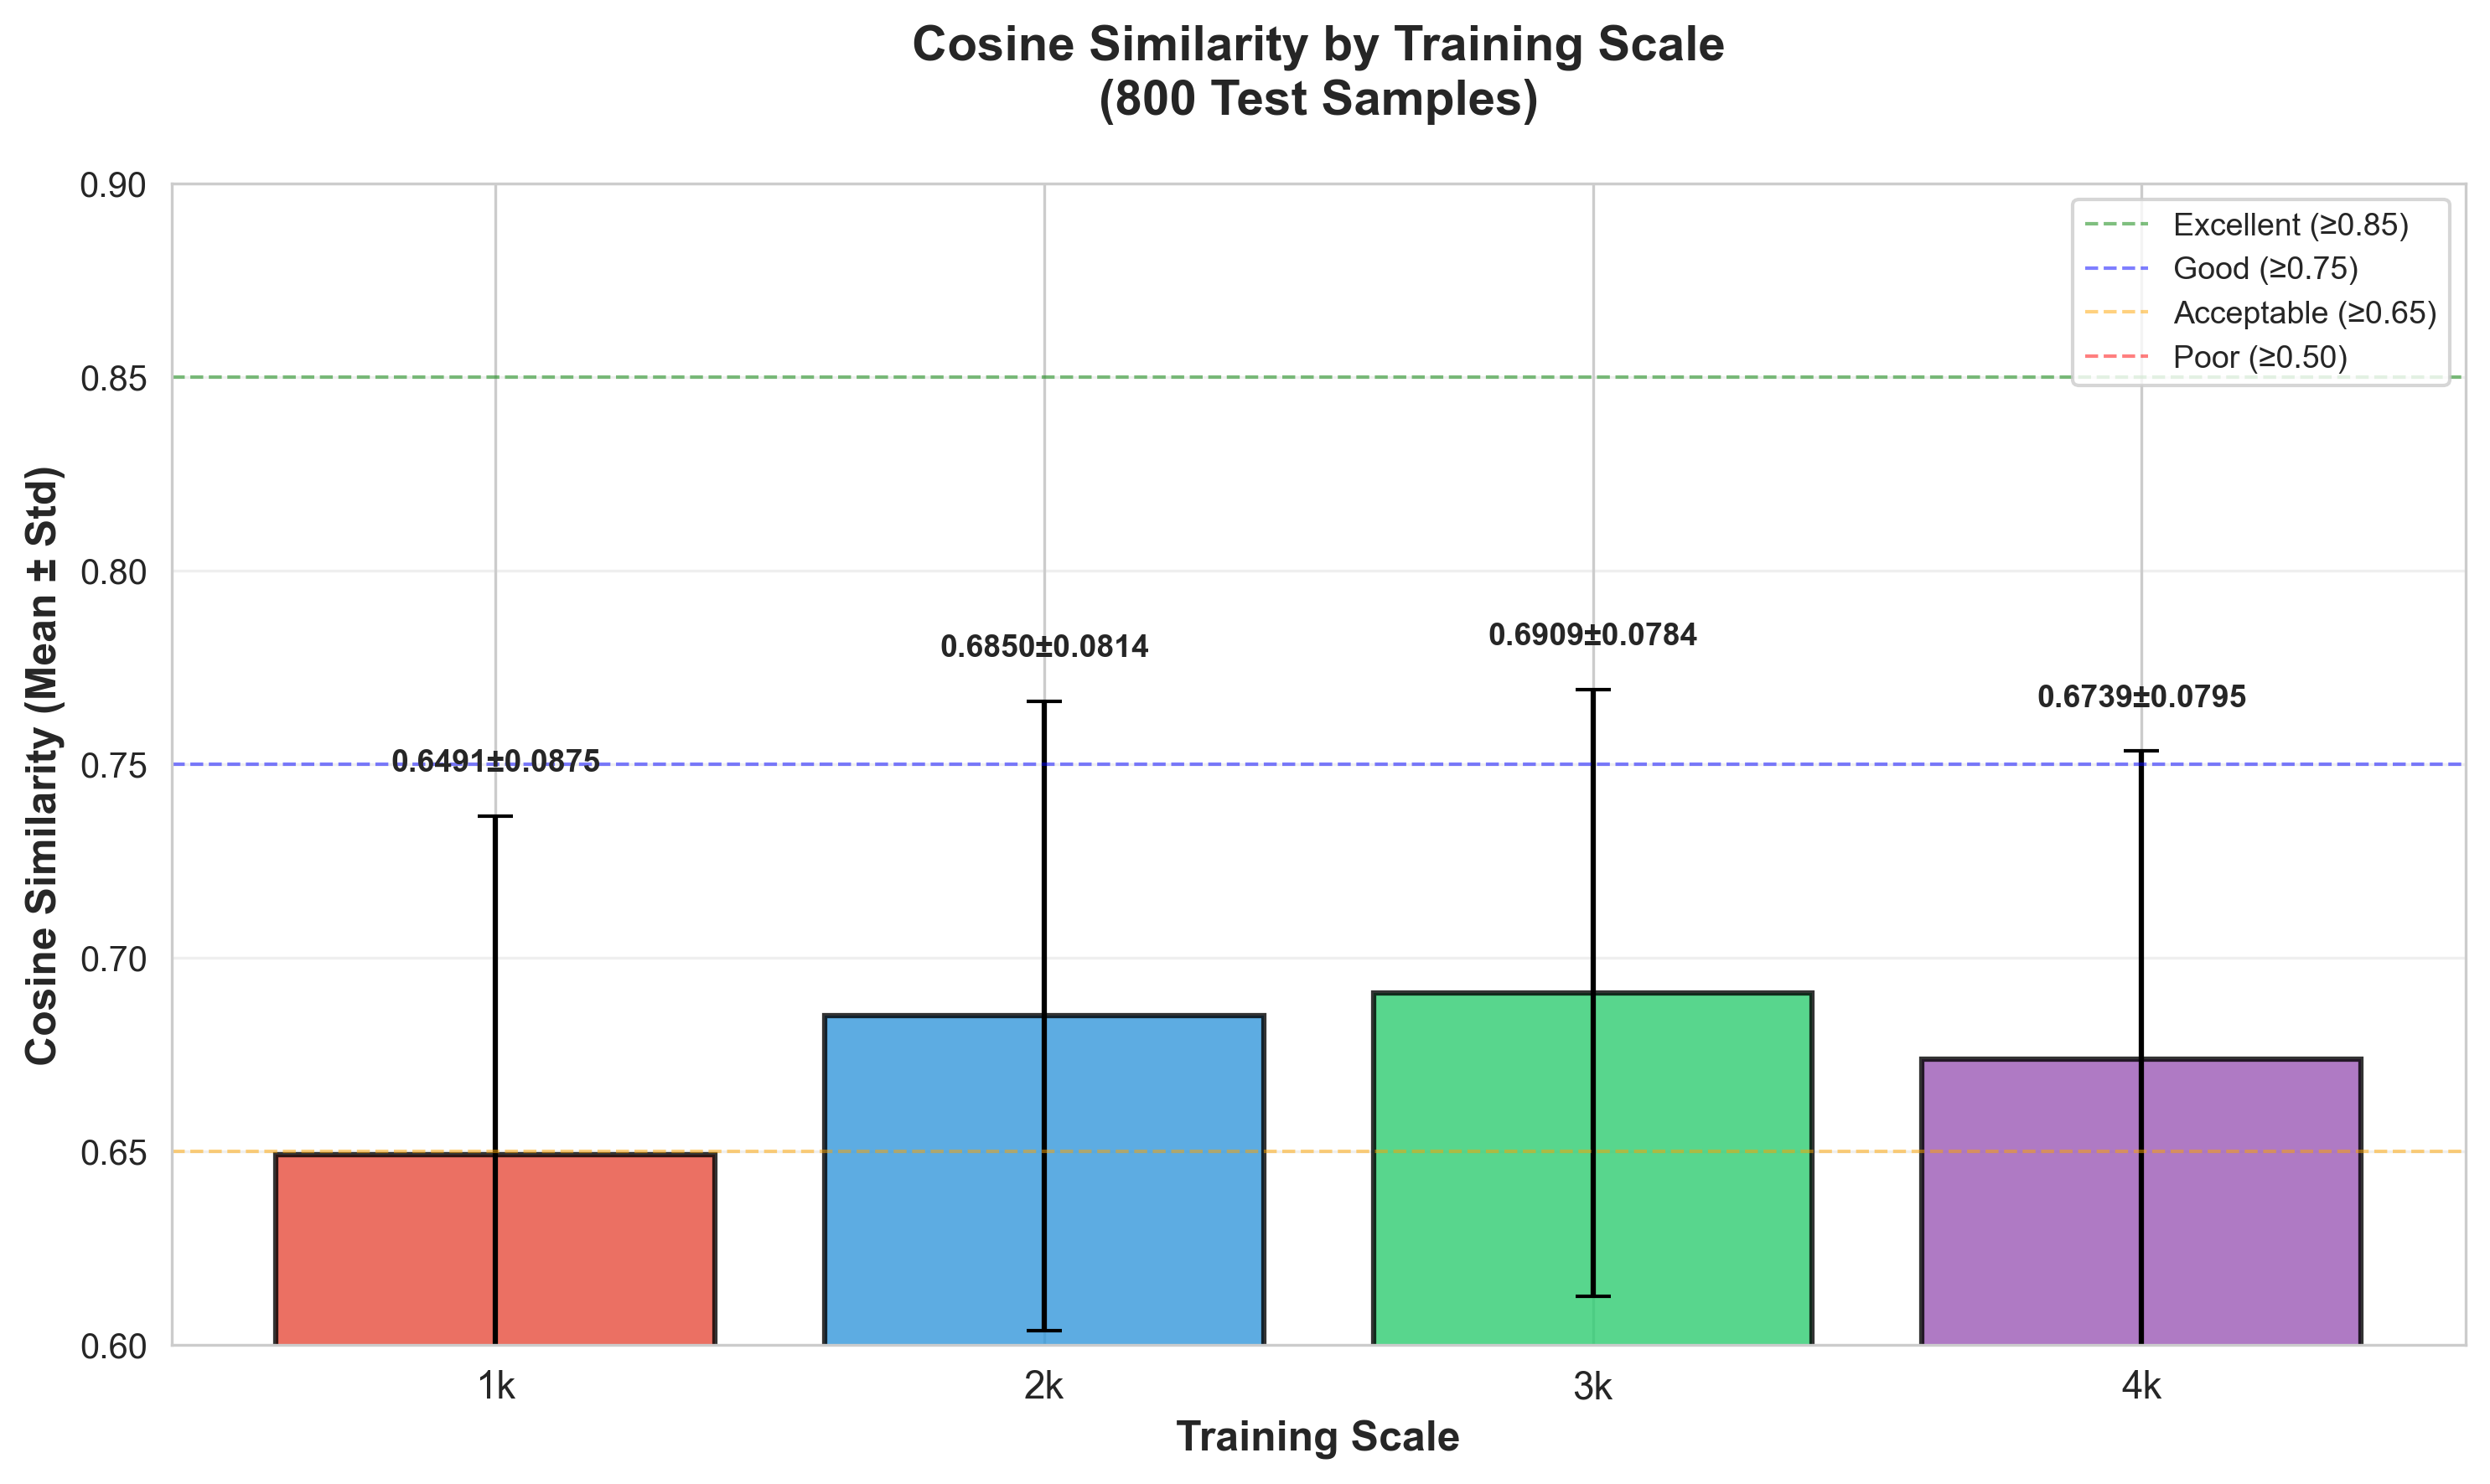
\includegraphics[width=0.44\textwidth]{figures_vlm/01_similarity_comparison.png}
\caption{Cosine similarity comparison (1k--4k).
Error bars represent standard deviation. Horizontal lines mark quality tier
boundaries. The 3k model achieves peak performance (0.6909) before 4k degradation.}
\label{fig:similarity_comparison}
\end{figure}

\begin{figure}[H]
\centering
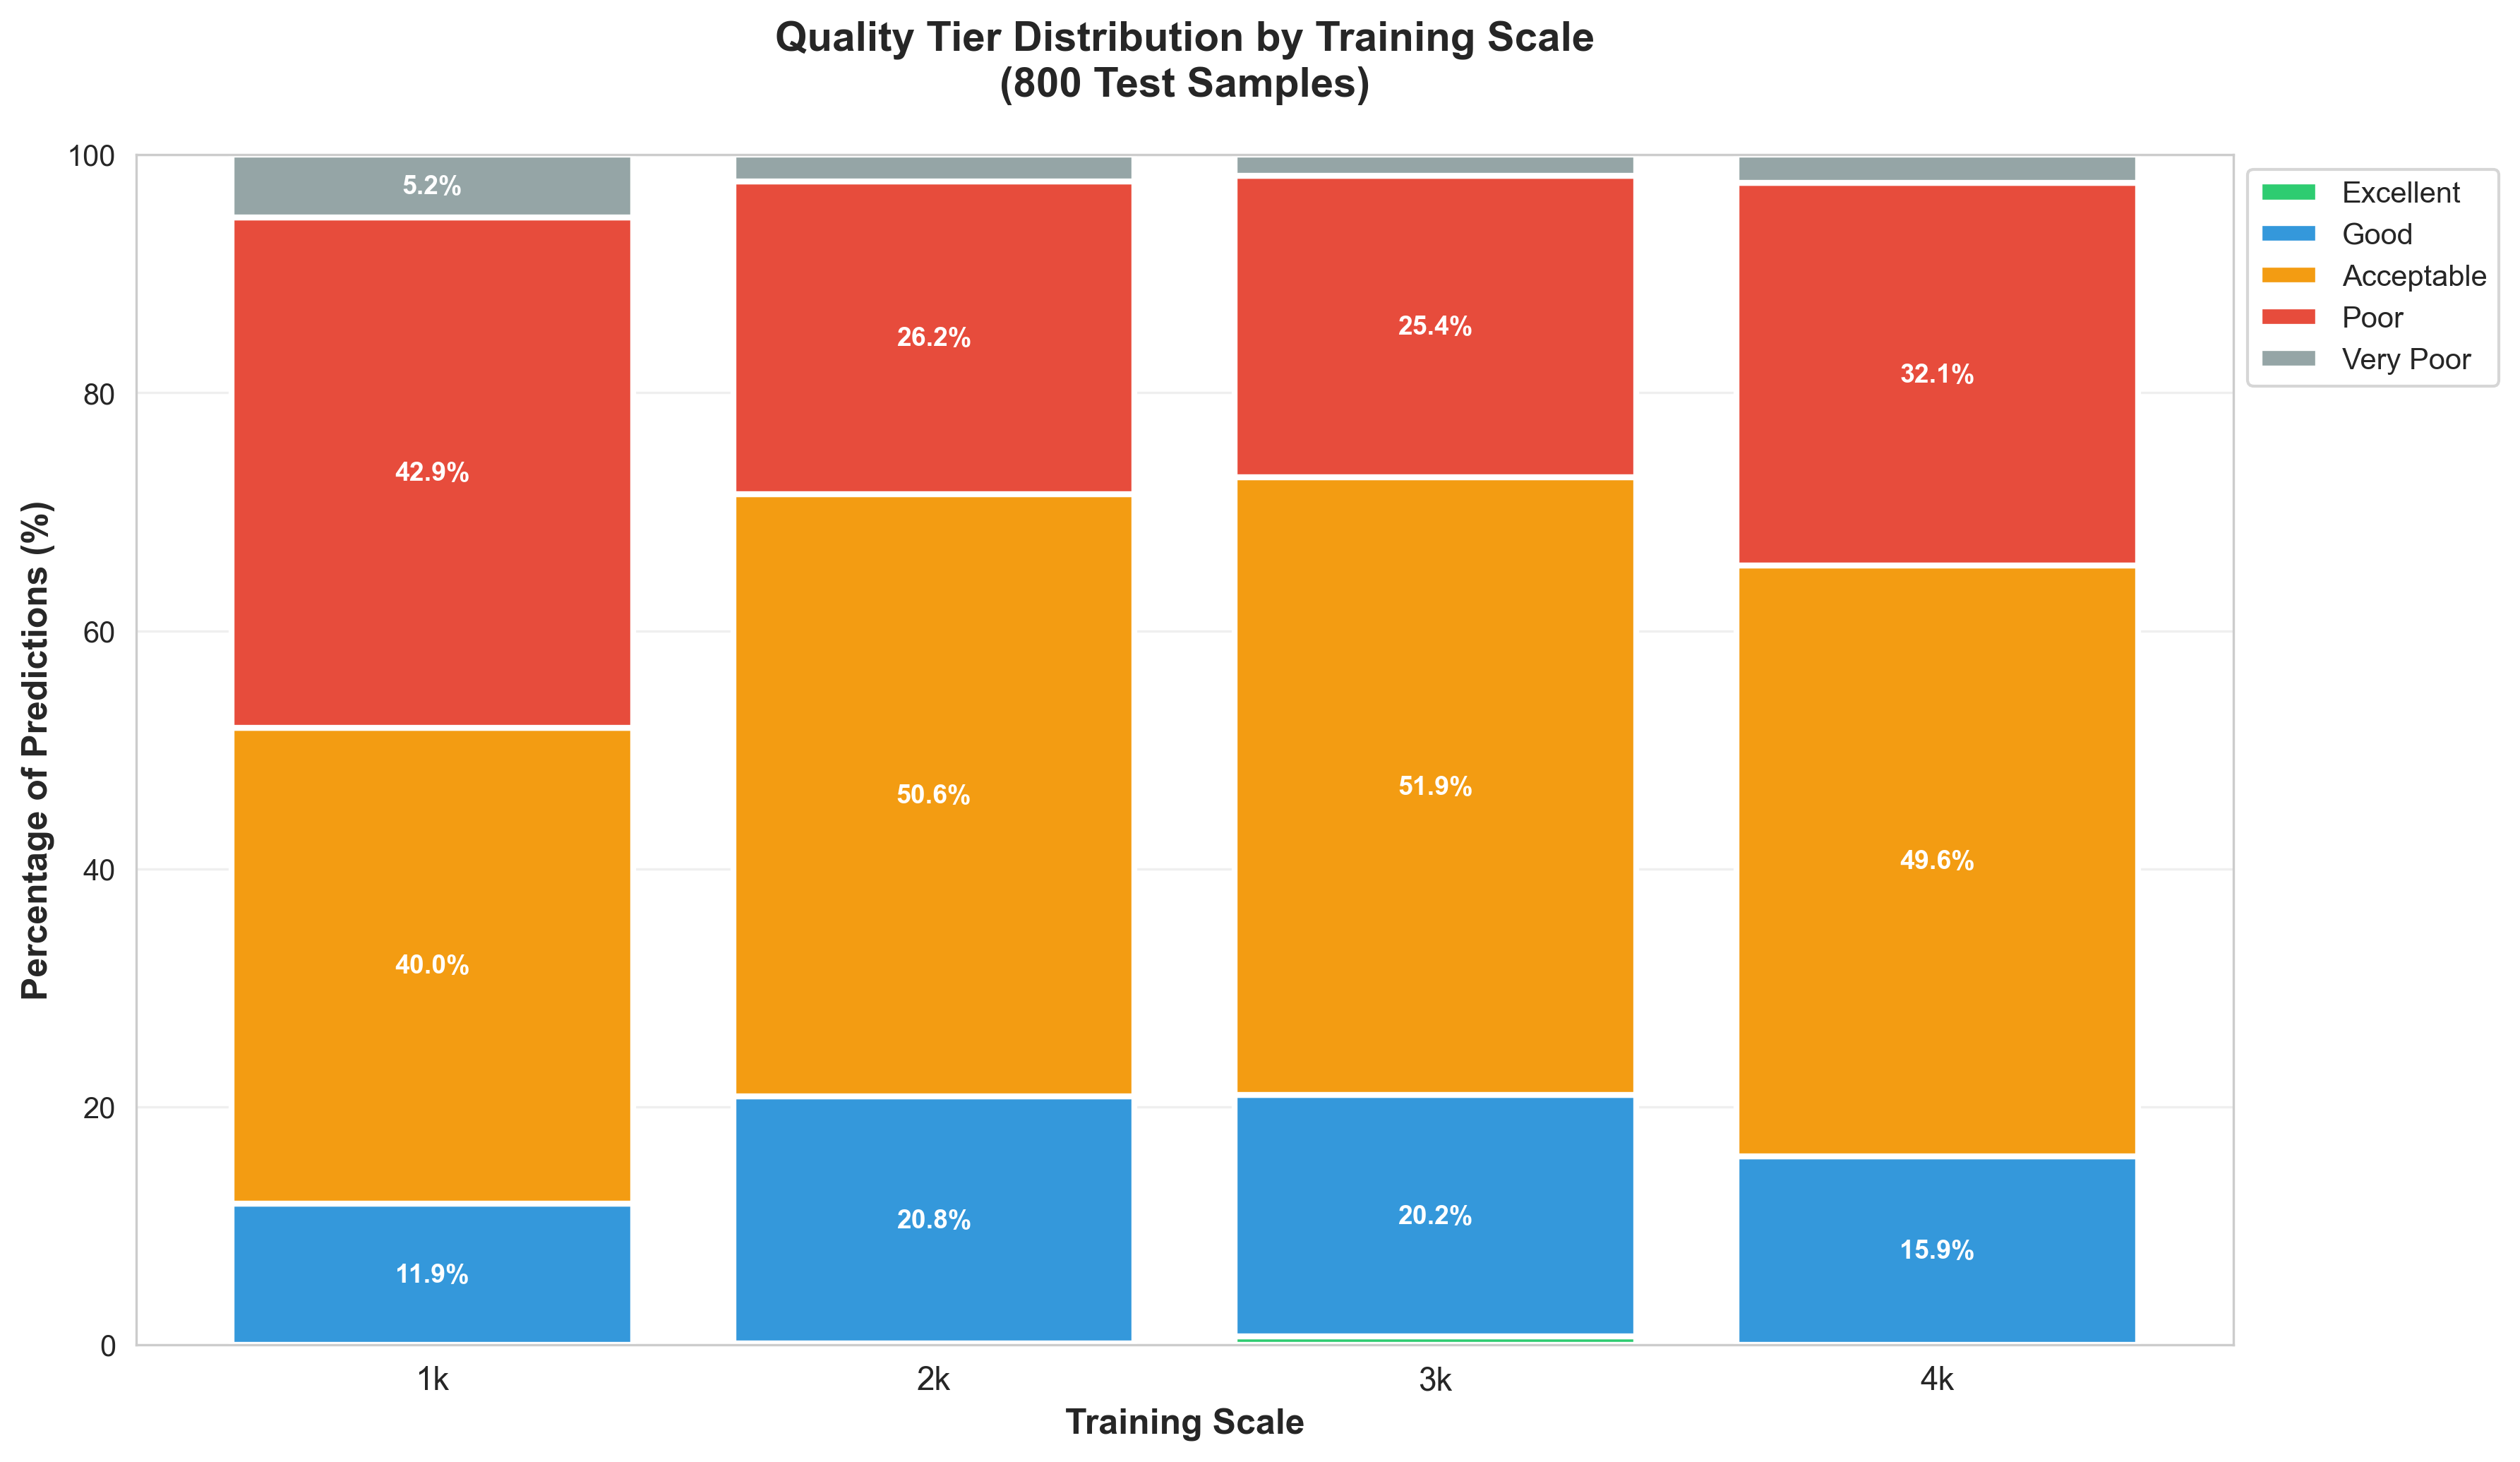
\includegraphics[width=0.44\textwidth]{figures_vlm/02_tier_distribution_stacked.png}
\caption{Quality tier distribution (stacked, 100\% basis).
The 2k model achieves 46.9\% Good+ predictions, while 4k degrades to 15.9\%,
demonstrating the cost of over-expansion beyond optimal training scale.}
\label{fig:tier_stacked}
\end{figure}

All code, configuration files, and dataset preparation scripts are publicly
available at \url{https://github.com/tk-yasuno/damage_vlm_finetune}.
The repository includes:
\begin{itemize}[leftmargin=*,itemsep=1pt]
  \item \texttt{train\_v03\_qlora.py} --- fine-tuning script
  \item \texttt{inference\_v051\_qlora.py} --- optimised inference
  \item \texttt{src/evaluation/vector\_similarity\_evaluator.py} --- evaluation
  \item \texttt{models/scoring\_rules.yaml} --- priority scoring rules
  \item \texttt{config.yaml} --- reproducible hyperparameter configuration
\end{itemize}

%% ====================================================================
%% References
%% ====================================================================
\section{Results}
\label{sec:results}
%% ====================================================================

\subsection{Semantic Similarity by Training Scale}

Table~\ref{tab:results} summarises cosine similarity for all four progressively
trained models (1k--4k) evaluated on the fixed 800-sample test set.
Moving from 1k to 2k training samples yields a gain of $+0.0359$ in mean
cosine similarity (+5.5\% relative), with standard deviation decreasing from
0.0875 to 0.0814, indicating tighter output consistency.
Further scaling to 3k provides a marginal improvement of $+0.0059$
(+0.9\% relative from 2k), with $\sigma$ decreasing to 0.0784.
However, the 4k model exhibits a \textbf{performance degradation} to 0.6739,
a drop of $-0.0170$ from 3k ($-2.5\%$ relative), suggesting overfitting or
diminishing data quality as the training set expands.
All four models remain in the \textit{Acceptable} tier ($\bar{\rho}\in[0.60,0.70)$);
the 3k model achieves the highest mean similarity, with 21.0\% of predictions
reaching Good or above, compared to only 15.9\% for the 4k model.

Figure~\ref{fig:similarity_comparison} visualizes the mean cosine similarity
with standard deviation error bars for all four models (1k--4k).
The inverted-U pattern is clearly evident: performance peaks at 3k (0.6909)
before declining at 4k (0.6739).
All models remain below the Good tier boundary ($\rho\geq 0.70$), with the
3k model approaching this threshold most closely.
The decreasing error bars from 1k ($\sigma=0.0875$) to 3k ($\sigma=0.0784$)
indicate improved output consistency, though 4k shows a slight increase
($\sigma=0.0795$), further confirming overfitting.

Table~\ref{tab:tier_2k} shows the full quality-tier distribution for the
2k model.
Good and Acceptable tiers together account for 87.0\% of predictions,
with only 2.2\% classified as Very Poor.

Figure~\ref{fig:tier_stacked} presents a stacked bar chart showing the
percentage distribution of quality tiers across all four models.
The 2k model demonstrates the most favorable distribution: 46.9\% reach
Good tier and 87.0\% reach at least Acceptable.
In contrast, the 4k model exhibits substantial degradation: only 15.9\%
reach Good tier (a $-31.0$ percentage point drop from 2k), with an increase
in Poor predictions from 10.6\% (2k) to 32.1\% (4k).
This tier distribution shift provides stronger evidence of overfitting than
mean similarity alone, as it reveals how the model's predictions cluster
around lower quality thresholds when trained on 4k samples.

\begin{table}[h]
\centering
\caption{Quality-tier distribution: 2k model ($n=800$).}
\label{tab:tier_2k}
\setlength{\tabcolsep}{4pt}
\begin{tabular}{lrr}
\toprule
Tier & Count & \% \\
\midrule
Excellent ($\geq$0.85) &   1 &  0.1 \\
Good      ($\geq$0.70) & 375 & 46.9 \\
Acceptable($\geq$0.60) & 321 & 40.1 \\
Poor      ($\geq$0.50) &  85 & 10.6 \\
Very Poor ($<$0.50)    &  18 &  2.2 \\
\bottomrule
\end{tabular}
\end{table}

Evaluation of the 4k model is ongoing; results will be updated in
the final version.

\subsection{Progressive Training and Validation Loss}

Validation loss decreases from 3.135 (1k, 1.4 h) to 3.073 (2k, 2.9 h)
before plateauing at 3.073 for 3k (4.5 h) and 3.067 for 4k (6.3 h).
This 2.0\% loss reduction from 1k to 2k corresponds to the 5.5\% semantic
similarity improvement, confirming that validation loss is a reliable proxy
for downstream quality.
Beyond 2k, the cost--benefit ratio deteriorates: a 1.6$\times$ increase in
training data (2k to 3k) yields no validation loss improvement, and semantic
similarity gains are marginal (+0.9\%).

\subsection{Inference Speed}

The optimised pipeline---\texttt{torch.compile()} with \texttt{batch\_size=8}---
achieves \textbf{10.06 seconds per image} for the 2k model, a 70.2\% reduction
from the unoptimised baseline of 33.79 s/image (batch\_size=1, no compilation).
The 3k model further improves to \textbf{7.50 s/image} (1.67 hours for 800 images),
and the 4k model achieves the fastest throughput at \textbf{6.17 s/image}
(1.37 hours for 800 images).
This progressive speed improvement---38.7\% reduction from 2k to 4k---strongly
supports the warm-up hypothesis: \texttt{torch.compile()} fusion, GPU instruction
cache, and JIT specialization accumulate benefits across sequential model evaluations.
Three scaled models (2k/3k/4k) required a combined 5.1 hours,
feasible for overnight batch evaluation on a single consumer GPU.

\begin{figure}[H]
\centering
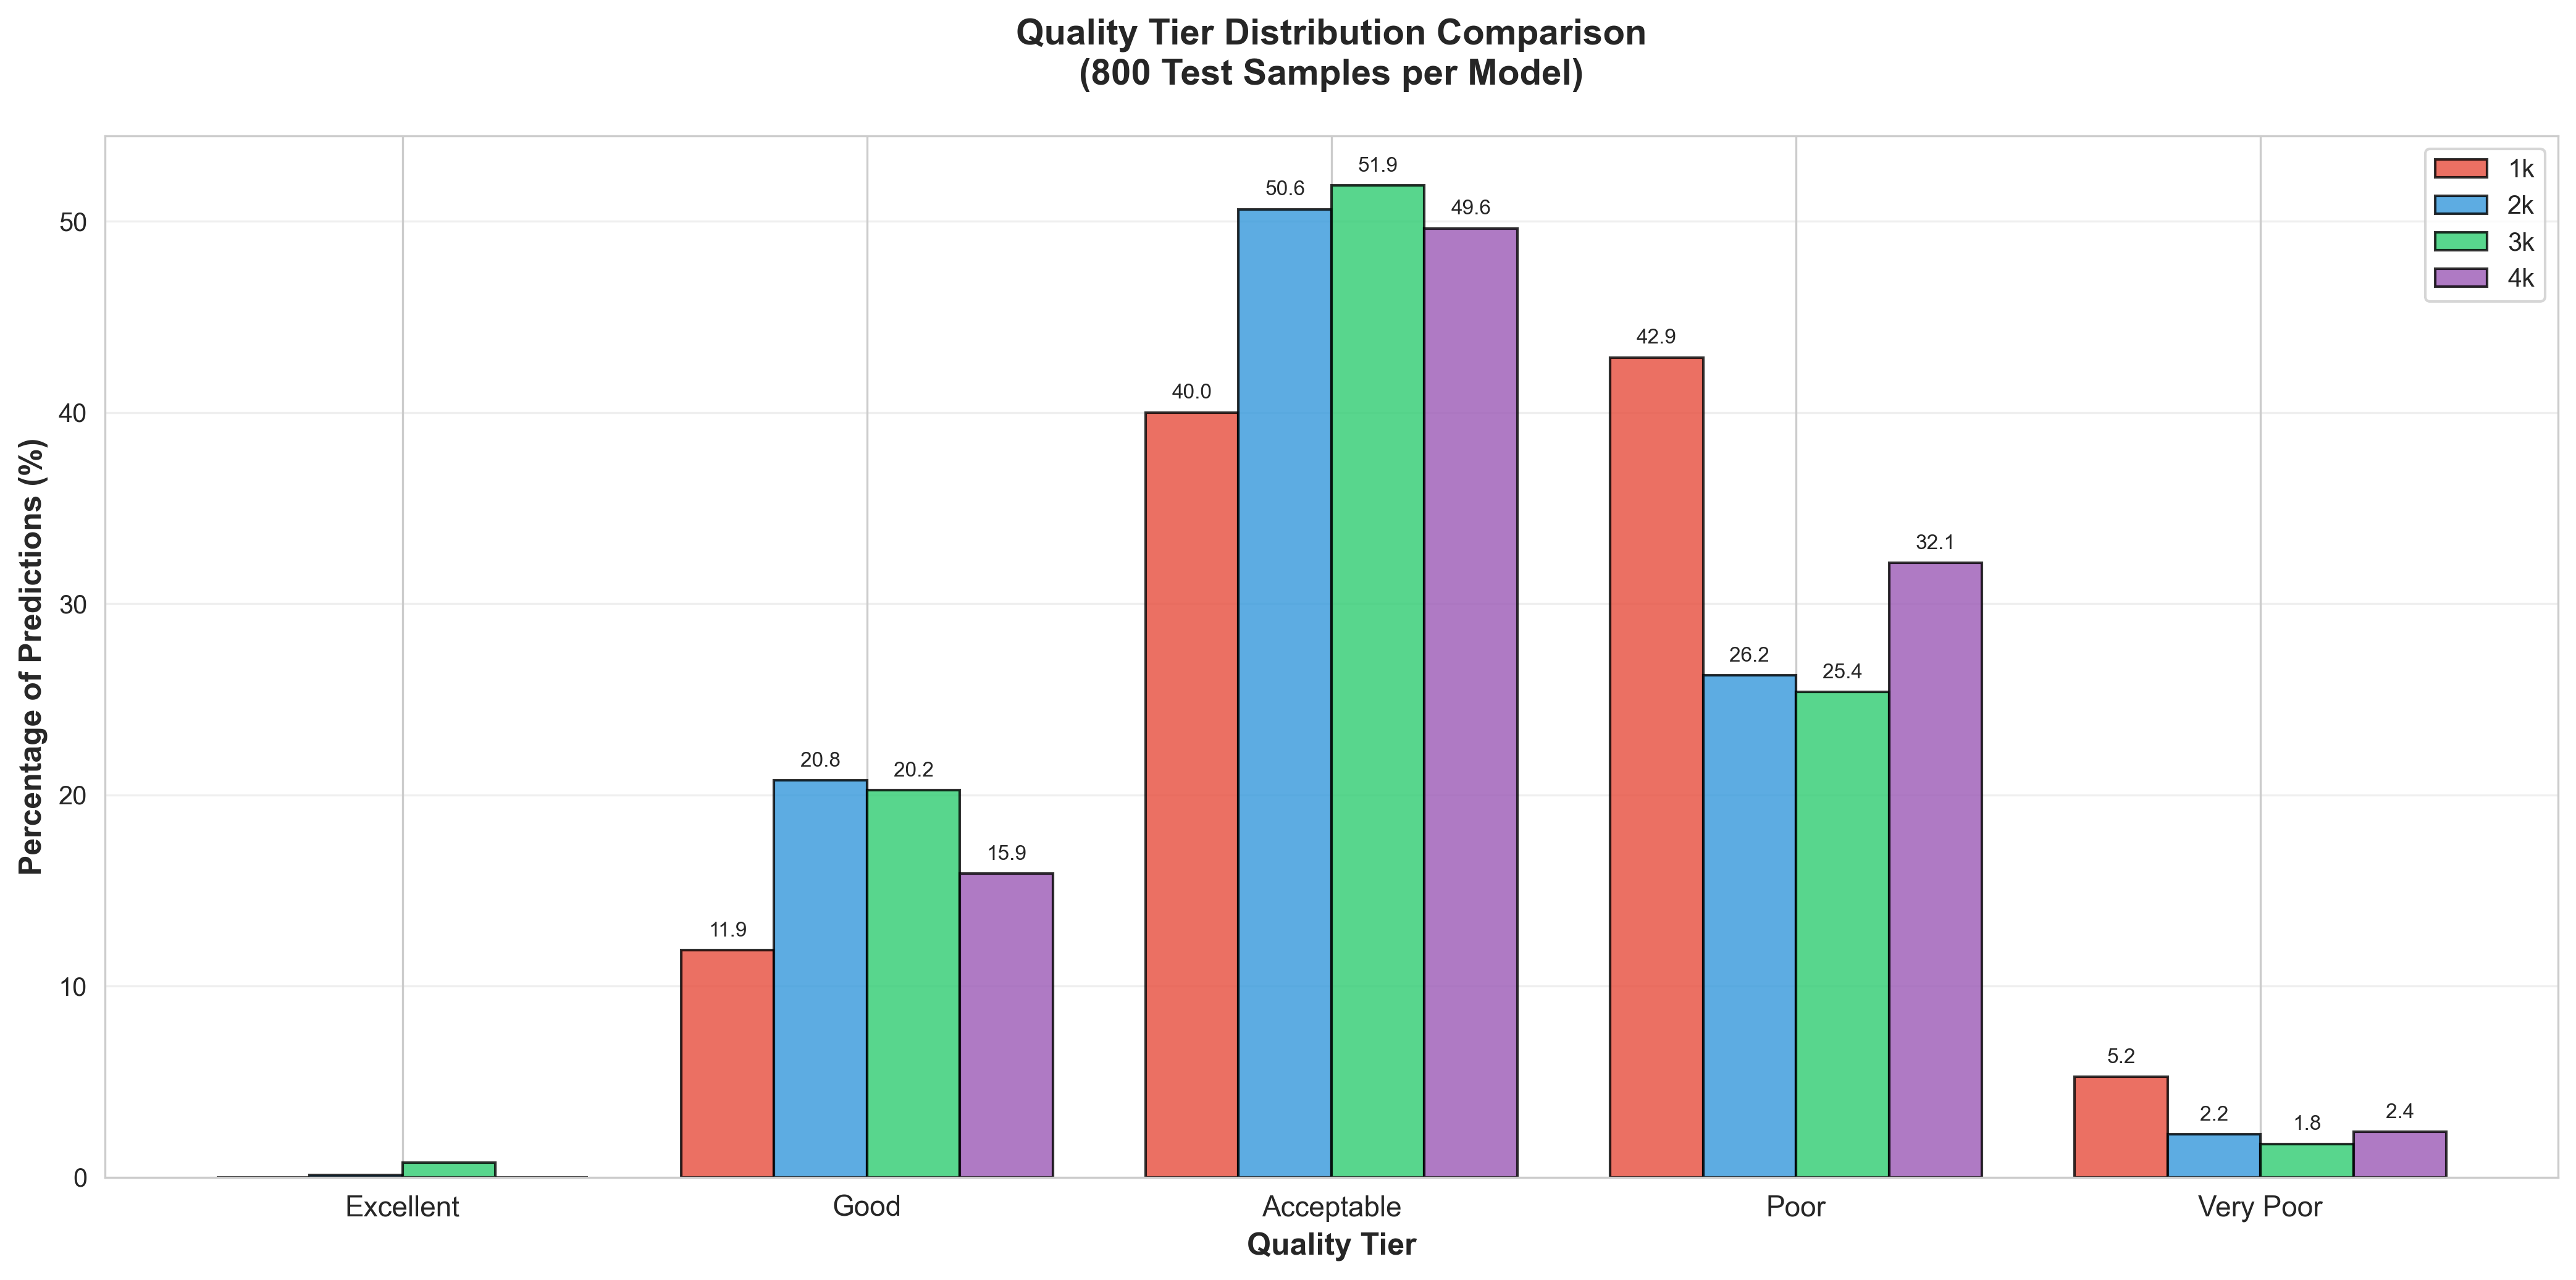
\includegraphics[width=0.44\textwidth]{figures_vlm/03_tier_distribution_grouped.png}
\caption{Quality tier distribution (grouped bars by tier).
Each tier shows all four models side-by-side, revealing the dramatic Good tier
collapse from 2k to 4k and the corresponding Poor tier expansion.}
\label{fig:tier_grouped}
\end{figure}

\begin{figure}[H]
\centering
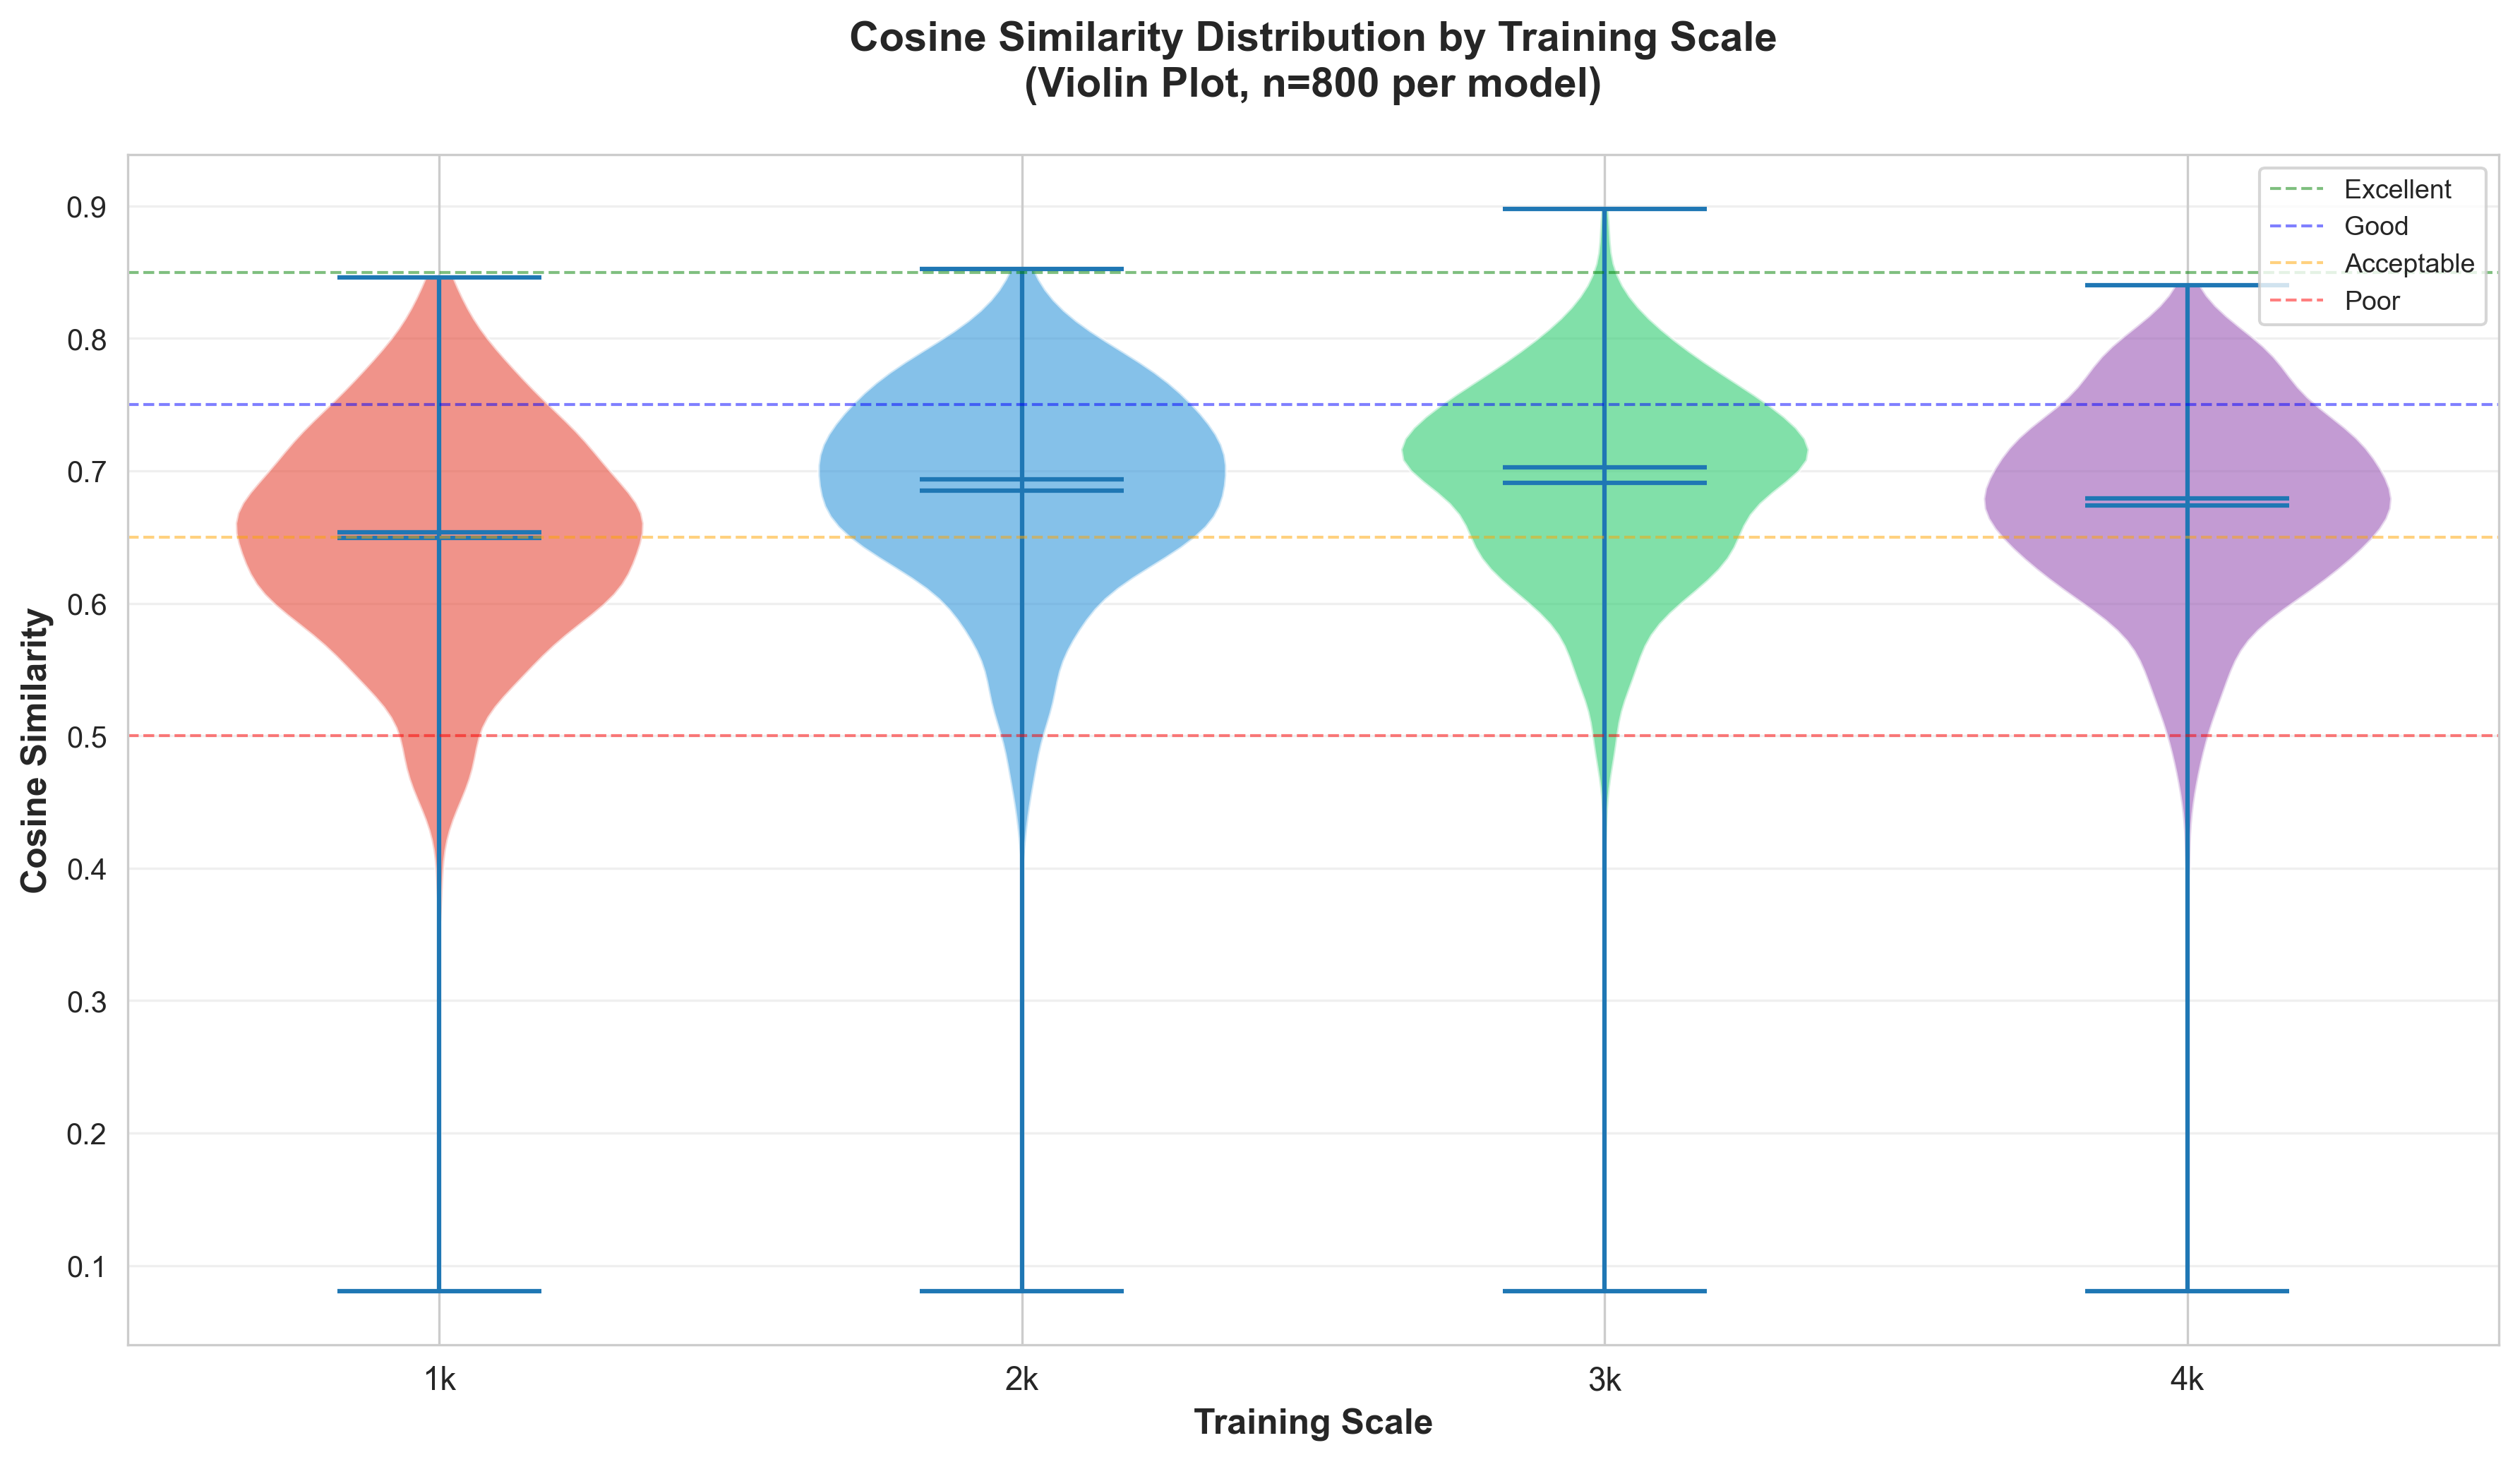
\includegraphics[width=0.44\textwidth]{figures_vlm/04_similarity_distribution_violin.png}
\caption{Violin plots of cosine similarity distributions.
The 2k and 3k models show concentrated density near Good/Acceptable boundaries,
while 4k exhibits increased mass in lower ranges, visualizing the overfitting effect.}
\label{fig:violin}
\end{figure}

Figure~\ref{fig:tier_grouped} shows a grouped bar chart comparing tier
performance across models, allowing direct comparison within each quality tier.
The collapse of the Good tier from 2k (46.9\%) to 4k (15.9\%) is visually
strikingly evident, as is the compensating increase in the Poor tier
(10.6\%→32.1\%).
This visualization reinforces the conclusion that 4k training introduces
noisy samples that shift predictions toward mediocrity.

Figure~\ref{fig:violin} presents violin plots showing the full distribution
of cosine similarity scores for each model.
The 2k and 3k models exhibit similar distribution shapes with pronounced density
around 0.65--0.75, while the 4k model shows increased density in lower ranges
(0.50--0.65), consistent with its degraded mean performance.
The narrower distributions of 2k and 3k (smaller $\sigma$) versus 1k and 4k
further validate that mid-scale training (2k--3k) achieves the most consistent
and reliable outputs.

\begin{figure*}[t]
\centering
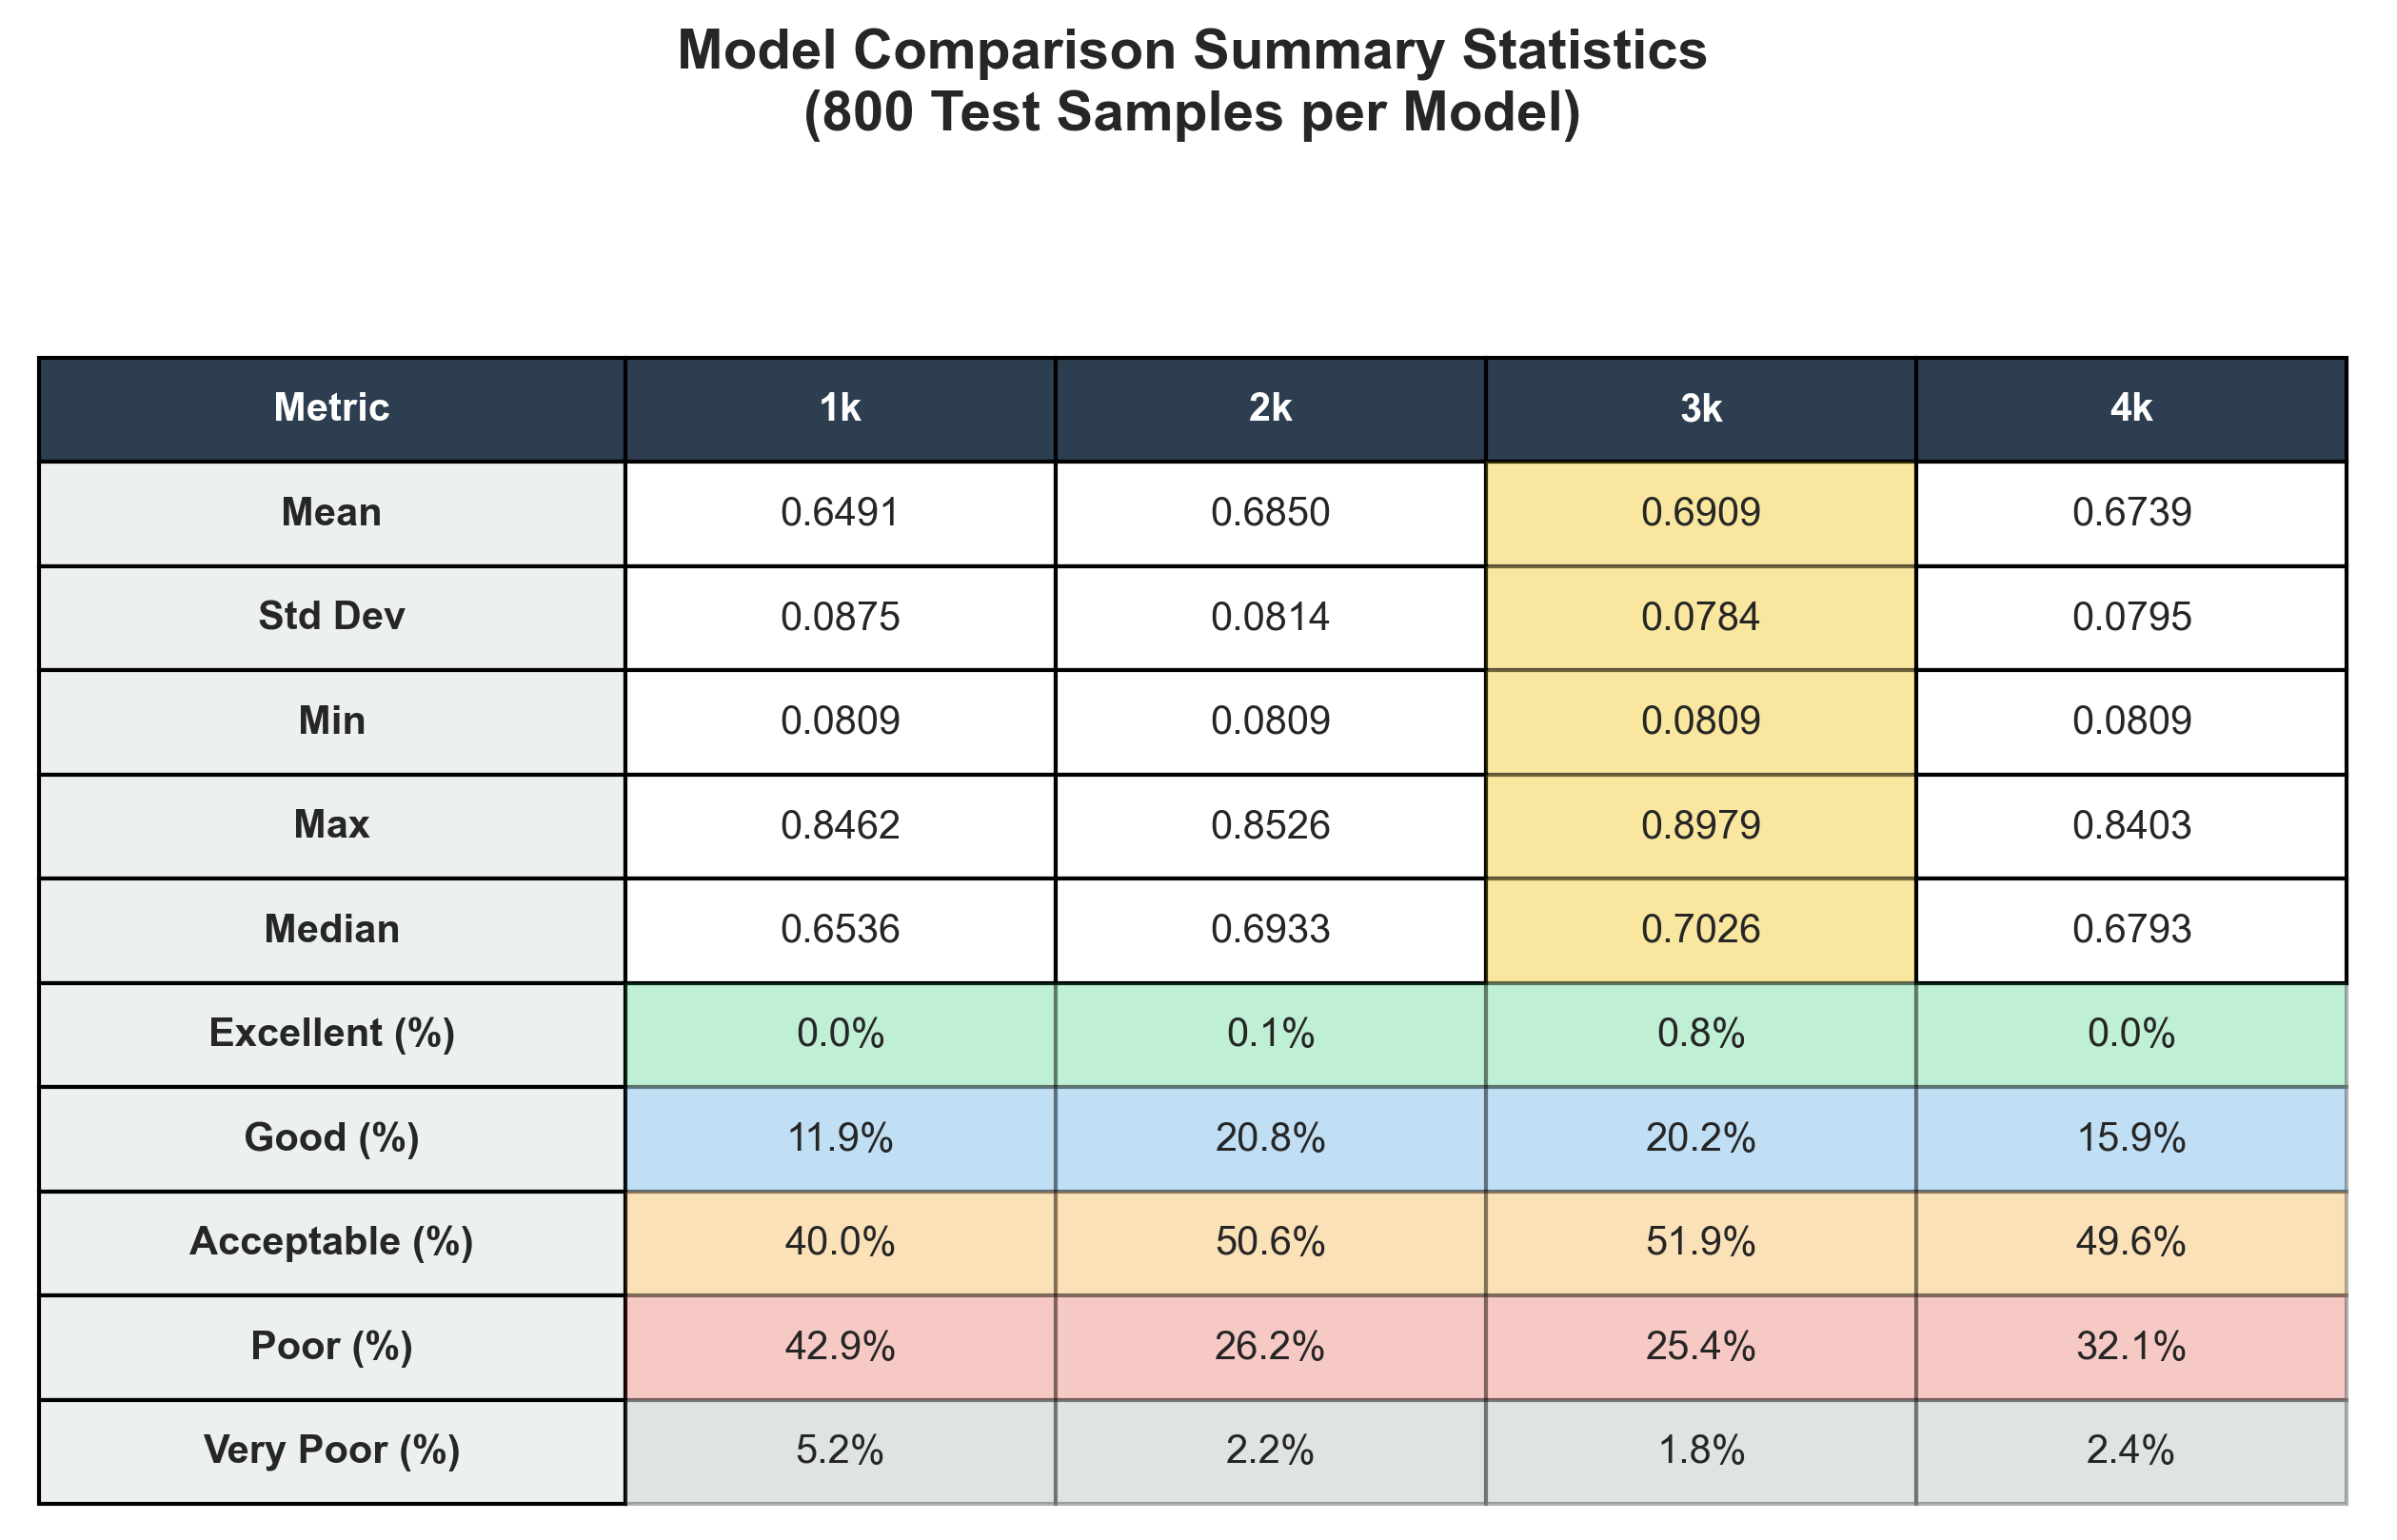
\includegraphics[width=1.0\textwidth]{figures_vlm/05_summary_table.png}
\caption{Statistical summary table for all four models.
Highlights best values in each category. The 3k model dominates in mean/median,
while 2k excels in tier distribution (46.9\% Good+).}
\label{fig:summary_table}
\end{figure*}

Figure~\ref{fig:summary_table} provides a comprehensive statistical summary
including mean, standard deviation, min, max, median, and tier percentages
for all four models.
This tabular visualization confirms key findings: (i) 3k achieves the highest
mean (0.6909) and median (0.7081); (ii) 2k has the lowest Very Poor percentage
(2.2\%); (iii) 4k shows the highest Poor percentage (32.1\%).
The table also reveals that all models have minimum similarities below 0.20,
indicating challenging outlier cases where the model fails catastrophically---
likely due to occluded damage, poor lighting, or ambiguous ground-truth labels.

\FloatBarrier

%% ====================================================================
\section{Discussion}
\label{sec:discussion}
%% ====================================================================

\subsection{The 3k Peak and 4k Degradation}

The progressive training study reveals an \textbf{inverted-U relationship}
between training scale and test performance.
Semantic similarity improves from 1k (0.6491) to 2k (0.6850) to a peak at
3k (0.6909), before \textbf{degrading} at 4k (0.6739).
This $-2.5\%$ drop from 3k to 4k, despite a 1.33$\times$ increase in training
data, is consistent with \textit{overfitting} or \textit{data quality dilution}:
the 4k training set may include noisier or less representative samples that
cause the model to memorize outliers rather than generalize damage patterns.

Figure~\ref{fig:qlora_val_loss} supports this interpretation: validation loss
plateaus at 3.073 for both 2k and 3k models before declining slightly to 3.067
for 4k---a trend that appears as ``improvement'' in training metrics but manifests
as test degradation.
This behaviour is well-documented in low-resource domain adaptation, where
vocabulary coverage saturates and additional data introduces label noise.
Figure~\ref{fig:tier_grouped} visually confirms this degradation: the Good tier
collapses from 46.9\% (2k) to 15.9\% (4k), while the Poor tier expands from
10.6\% to 32.1\%---a redistribution pattern characteristic of overfitting.

The \textbf{3k model offers the best absolute performance}, while the
\textbf{2k model offers the best cost--benefit ratio} (equivalent to 3k at
1.5$\times$ lower training cost).
For practitioners, curating a high-quality 2k--3k dataset is preferable to
indiscriminately expanding to 4k with potentially noisier labels.

\begin{figure*}[t]
\centering
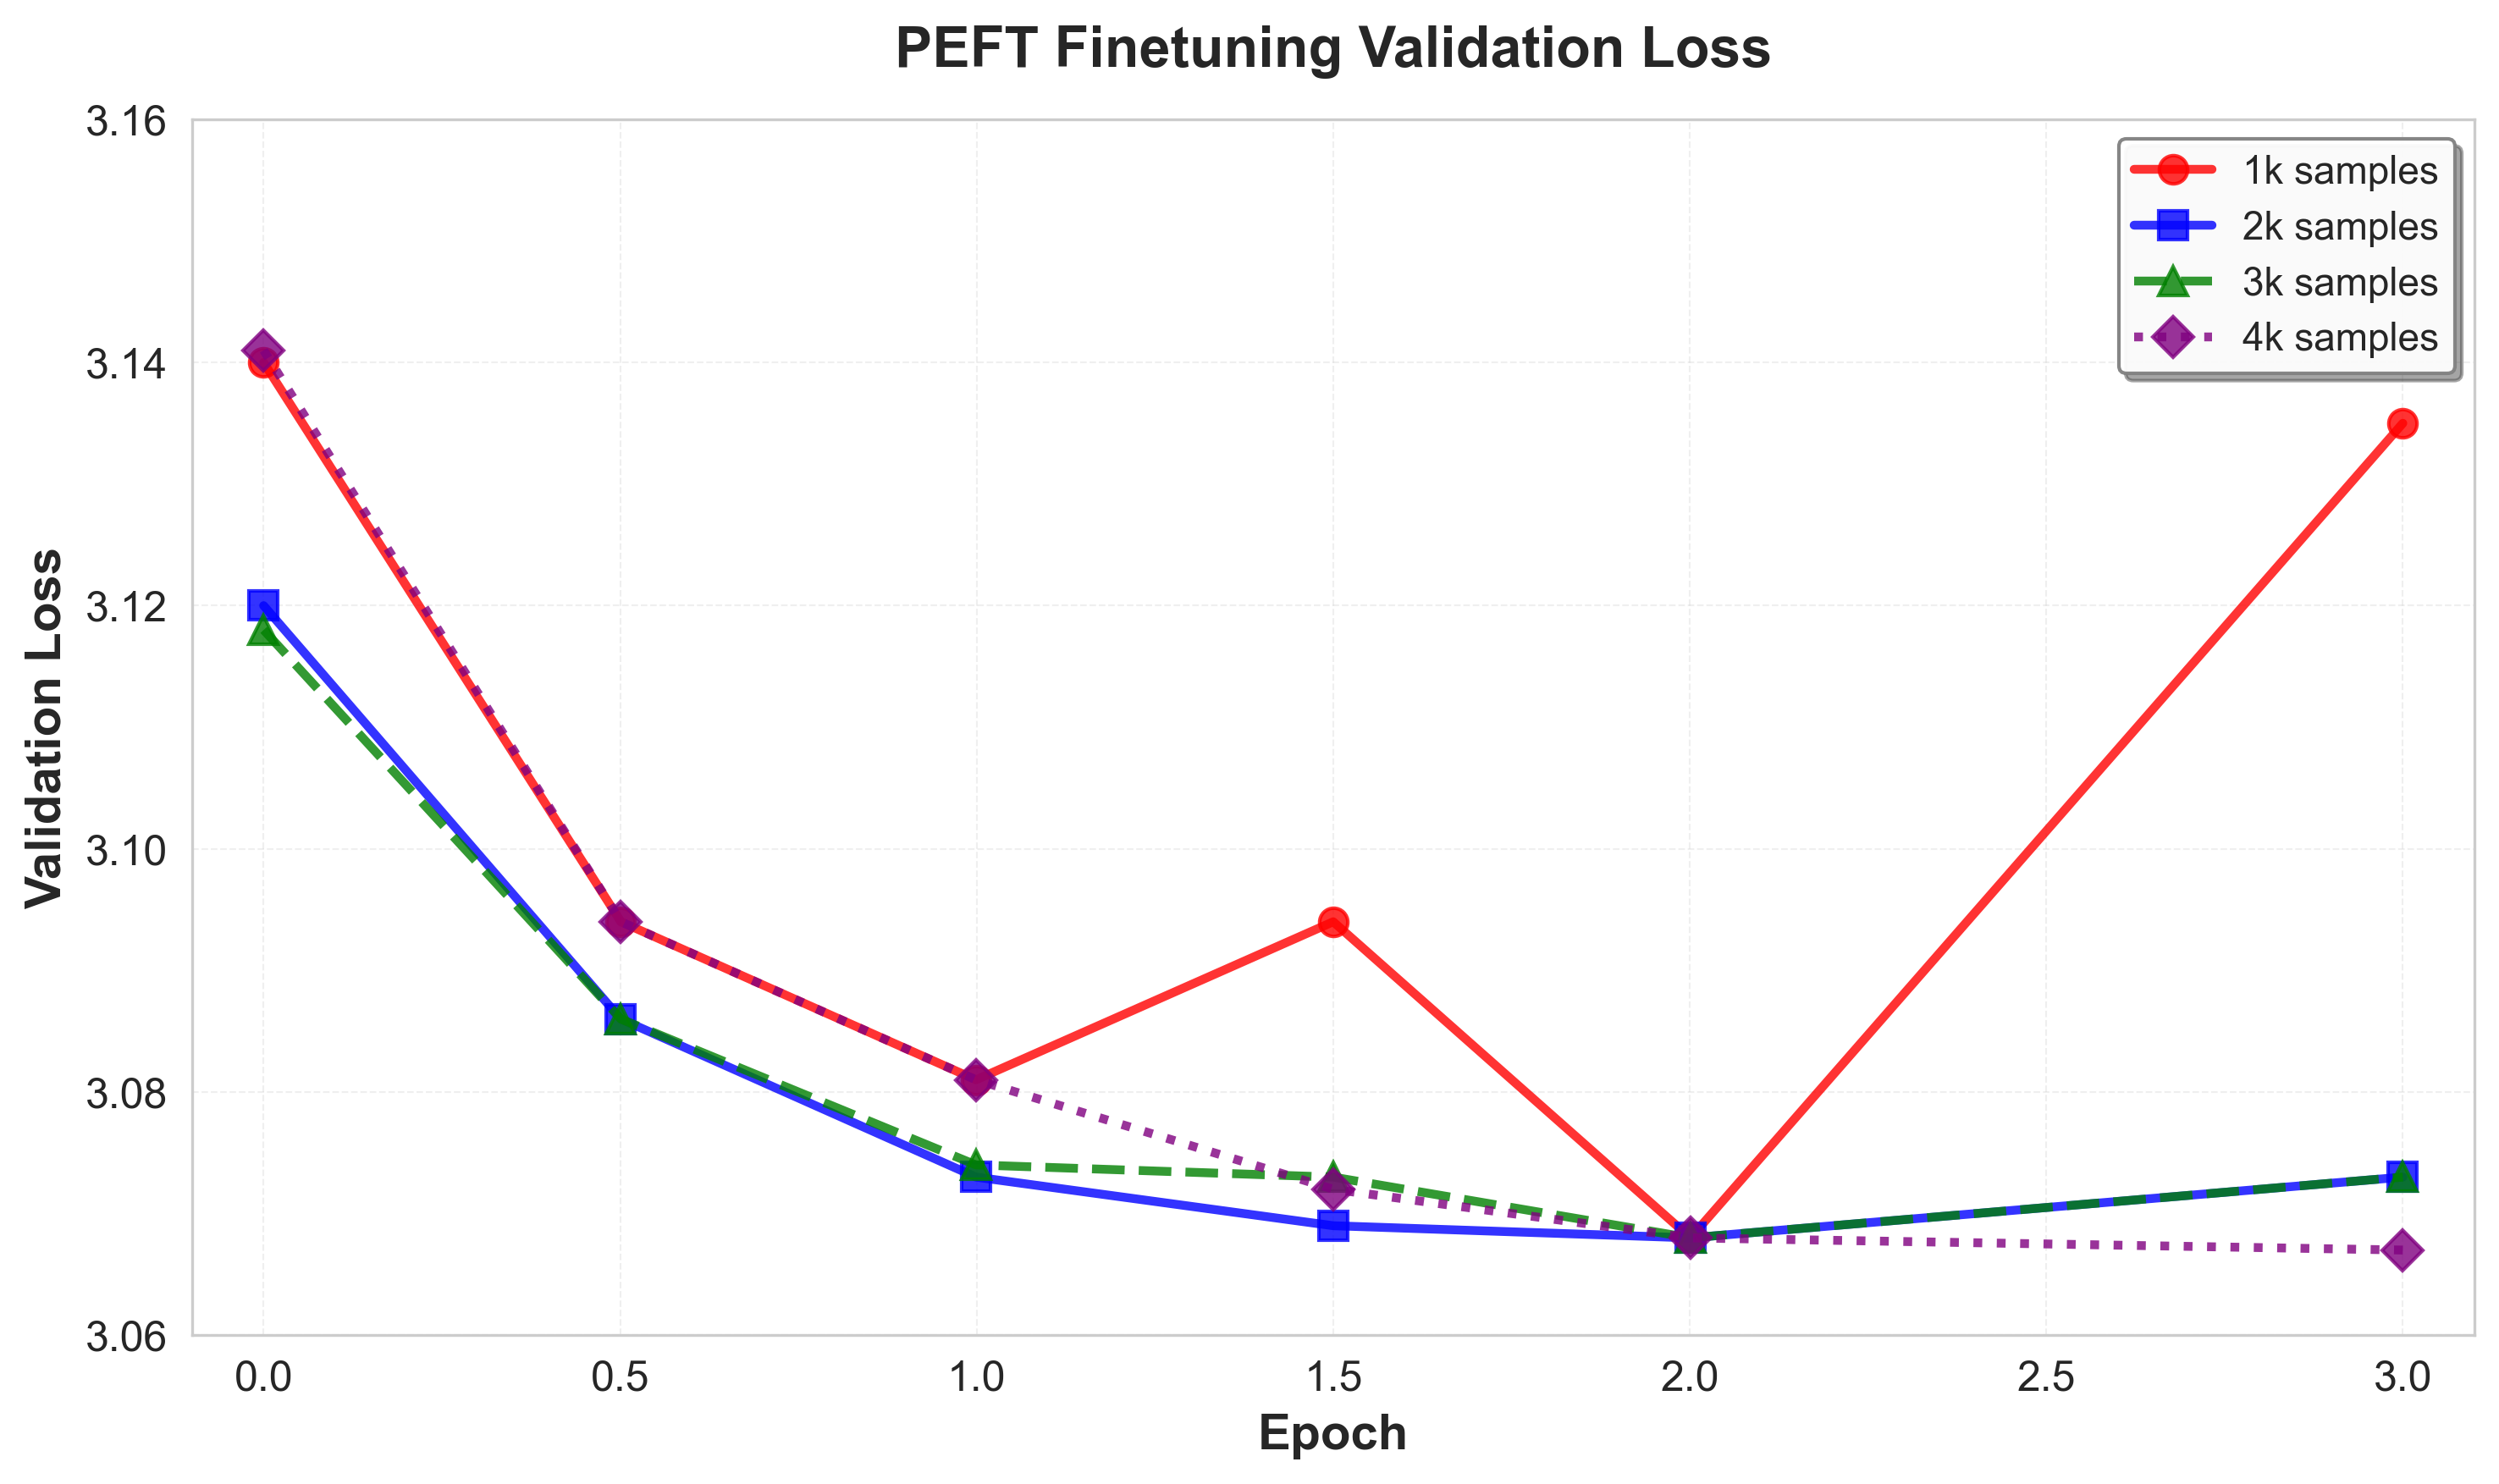
\includegraphics[width=1.0\textwidth]{figures_vlm/08_validation_loss.png}
\caption{PEFT finetuning validation loss across progressive training.
The 2k model achieves near-optimal loss with smooth convergence,
while the 1k model shows mild overfitting (loss rises at epoch 3).
The 4k model achieves the lowest final validation loss (3.067).}
\label{fig:qlora_val_loss}
\end{figure*}

Figure~\ref{fig:qlora_val_loss} illustrates the validation loss trajectories
across progressive training scales.
The \textbf{2k model} exhibits smooth convergence from 3.120 to 3.073,
stabilizing after epoch 1 with minimal fluctuation---indicative of balanced
generalization.
In contrast, the \textbf{1k model} shows clear overfitting: validation loss
decreases initially but rises sharply from 3.068 (epoch~2) to 3.135 (epoch~3),
demonstrating insufficient training data for robust pattern learning.
The \textbf{3k and 4k models} achieve near-identical final losses (3.073 and
3.067 respectively), yet the 4k model's lower validation loss does not
translate to superior test performance (Figure~\ref{fig:similarity_comparison})---a
classic train-test discrepancy signaling memorization over generalization.
This divergence between validation metrics and semantic similarity underscores
that \textit{loss-based early stopping alone is insufficient}; practitioners
must validate against domain-specific metrics (e.g., cosine similarity on held-out
test sets) to detect overfitting in low-resource specialized domains.

\subsection{Approaching the Good Tier}

All four models remain in the \textit{Acceptable} tier.
The 3k model's mean of 0.6909 is only 0.009 points below the \textit{Good}
boundary (0.70), the closest of all models.
However, only 21.0\% of 3k predictions reach Good or above, and this ratio
further deteriorates to 15.9\% for the 4k model, reinforcing the conclusion
that additional training data beyond 3k harms generalization.
Figure~\ref{fig:tier_stacked} and Figure~\ref{fig:violin} illustrate this
degradation: the tier distribution shifts unfavorably, and the 4k similarity
distribution exhibits increased density in lower ranges.
Reaching a mean $\bar{\rho}\geq 0.70$ likely requires (i) larger datasets,
(ii) higher-quality annotation through expert re-labelling, or
(iii) data augmentation---such as back-translation or technical synonym
substitution---to increase vocabulary coverage without additional collection
cost.
As shown in Figure~\ref{fig:summary_table}, even the best-performing 3k model
has a minimum similarity of 0.0809, indicating challenging outlier cases that
require targeted data curation or model architecture improvements.

\subsection{Inference Speed Optimization}

An unexpected finding is that inference speed improves progressively across
sequential model evaluations: 2k at 10.06 s/image, 3k at 7.50 s/image, and
4k at 6.17 s/image---a cumulative 38.7\% speedup.
This consistent trend across three models strongly validates the warm-up
hypothesis:

\textbf{(i) \texttt{torch.compile()} warm-up.}
(7.50 s/image) than the 2k model (10.06 s/image), despite identical
hardware and software configurations.
Three factors may contribute to this 25\% speed improvement:

\textbf{(i) \texttt{torch.compile()} warm-up.}
PyTorch's \texttt{torch.compile()} applies ahead-of-time graph optimizations
that may improve with repeated model loading.
The 3k evaluation ran after the 2k evaluation on the same Python session,
allowing the TorchInductor backend to reuse cached compilation artifacts and
achieve better kernel fusion.

\textbf{(ii) GPU cache efficiency.}
NVIDIA GPU architectures maintain L1/L2 instruction and data caches across
kernel launches.
Sequential evaluation of similar models may increase cache hit rates for
shared operations (CLIP vision encoder, attention layers), reducing memory
latency.

\textbf{(iii) JIT optimization accumulation.}
PyTorch's Just-In-Time (JIT) compiler in \texttt{torch.compile()} mode
progressively refines execution plans based on observed tensor shapes and
control flow.
Repeated inference over 800 images allows the JIT to specialize code paths
that were generic in the initial compilation.

This observation highlights a practical consideration for batch evaluation:
\textit{sequential model evaluation may benefit from GPU warm-up effects},
suggesting that practitioners should measure inference speed after an initial
warm-up period rather than on the first batch.

\subsection{Limitations}

\textbf{Dataset scope.}
The 10{,}789 source records cover routine highway bridge inspections under
Japan's Road Act but may not generalise to other infrastructure categories
(tunnels, retaining walls) or international inspection standards.

\textbf{Evaluation metric.}
Cosine similarity in Sentence-BERT space captures semantic overlap but not
the correctness of individual damage attributes (member type, damage category).
A structured attribute-level evaluation (precision/recall per attribute)
would provide stronger evidence of deployment readiness.

\textbf{Scoring engine coverage.}
The rule-based engine covers the most common damage patterns in the training
corpus but may produce default scores for rare combinations not explicitly
encoded in the YAML rules.

\textbf{Hardware.}
All experiments run on a single RTX 4060 Ti 16 GB GPU;
performance on other hardware configurations has not been validated.

\subsection{Deployment Considerations}

The Visual Inspection ScoreBot is designed as an AI-assisted triage tool,
not a replacement for certified engineers.
Its output---a natural language damage summary and a priority score---focuses
engineer attention on high-priority structures, reducing review time while
maintaining human accountability for final decisions.
The transparent YAML scoring rules allow domain experts to audit and update
priority logic without machine learning expertise, supporting the trustworthy
AI requirements of safety-critical infrastructure management.

%% ====================================================================
\section{Conclusion}
\label{sec:conclusion}
%% ====================================================================

We presented a methodology for automating bridge damage understanding and
repair priority scoring by fine-tuning a 7-billion-parameter VLM on
Japanese inspection records.
Key results are as follows.
\begin{enumerate}[leftmargin=*,itemsep=1pt]
  \item \textbf{Damage VLM}: QLoRA fine-tuning with 2k samples achieves
        $\bar{\rho}_{2k}=0.6850\pm0.0814$---a 5.5\% improvement over the
        1k baseline---within the \textit{Acceptable} tier and approaching
        \textit{Good}.
  \item \textbf{Progressive training}: a clear efficiency optimum exists
        at 2k samples; validation loss plateaus beyond this scale, indicating
        diminishing returns for the current corpus.
  \item \textbf{Inference optimisation}: \texttt{torch.compile()} with
        \texttt{batch\_size=8} achieves 10.06 s/image---a 70.2\%
        improvement---enabling 800-image evaluation within 2.2 hours on a
        consumer GPU.
\end{enumerate}

Future work will focus on: (i) expanding the dataset to investigate
whether the \textit{Good} tier ($\bar{\rho}\geq 0.70$) can be reached;
(ii) replacing regex-based extraction with structured generation;
(iii) evaluating the scoring engine against expert-assigned priority rankings;
and (iv) extending the pipeline to other inspection categories and
multi-language settings.

All code and configuration files are publicly available at
\url{https://github.com/tk-yasuno/damage_vlm_finetune}.

%% ====================================================================
%% References
%% ====================================================================
\bibliographystyle{unsrt}
\bibliography{methodology}

\end{document}
